\documentclass[9pt,twocolumn,twoside,lineno]{gsajnl}

\newcommand{\ra}{\rightarrow}
\newcommand{\afs}[2]{\Phi_{#1}^{(#2)}}
\newcommand{\afsPsi}[2]{\Psi_{#1}^{(#2)}}
\newcommand{\cond}{\middle\vert}
\newcommand{\dslash}{/\!\!/}
\newcommand{\Coalc}[4]{\begin{bmatrix}#1\dslash #2 \\ #3\dslash #4 \end{bmatrix}}

\newcommand{\CC}{\mathcal{C}}
\newcommand{\ms}{\mathcal{S}}
\newcommand{\Var}{\operatorname{Var}}

\newcommand{\sgcomment}[1]{\textcolor{blue}{SG: #1}}

\articletype{inv}

\title{ Taming strong selection with large sample sizes }

\author[$\ast$]{Ivan Krukov}
\author[$\ast$]{Simon Gravel}

\affil[$\ast$]{Genome Center, Department of Human Genetics, McGill University, Montreal, Canada}
\keywords{Coalescent; Strong selection; Allele-Frequency spectrum}

\runningtitle{Taming strong selection with large sample sizes}
\runningauthor{Krukov and Gravel}

\begin{abstract}

The fate of mutations and the genetic load of populations depend on the relative importance of
genetic drift and natural selection. In addition, the accuracy of numerical models of evolution
depends on the strength of both selection and drift: strong selection breaks the assumptions of
the nearly neutral model, and drift coupled with large sample sizes breaks
Kingman's coalescent model.

Thus, the regime with strong selection and large sample sizes, relevant to the study of pathogenic
variation, appears particularly daunting.  Surprisingly, we find that the interplay of drift
and selection in that regime can be used to define approximately closed recursions for the
distribution of allele frequencies that are accurate well beyond the strong selection limit (i.e., for $Ns\gg 1$).

Selection becomes more analytically tractable when the sample size $n$ is larger than twice the
population-scaled selection coefficient: $n \ge 2Ns$ ($4Ns$ in diploids). That is, when the
expected number of coalescent events in the sample is larger than the number of selective events.  We
construct the relevant transition matrices, show how they can be used to accurately compute
distributions of allele frequencies, and show that the distribution of deleterious allele frequencies is  sensitive to details of the evolutionary model.  

\end{abstract}

\begin{document}

\maketitle
\thispagestyle{firststyle}
\marginmark
\firstpagefootnote

\section{Introduction}
\label{sec_introduciton}

The allele frequency spectrum (\textit{AFS}) is an important summary of genetic diversity that is
commonly used to infer demographic history and natural selection (\textit{e.g.}
\cite{GutenkunstEtAl2009, KammEtAl2017, JouganousEtAl2017}). Given a demographic scenario of
population size histories and patterns of migration, these approaches use versions of the diffusion
approximation or coalescent simulations to obtain a predicted \textit{AFS}. By comparing
predictions to the observed \textit{AFS}, one can compute likelihoods for different demographic
scenarios. These approaches share two drawbacks.

First, the \textit{AFS} calculations can be time consuming for large sample sizes.  Some efficient
computational shortcuts can be used (e.g., \cite{fastsimcoal2, KammEtAl2017}) but these often
require neutrality.  In the presence of natural selection, available methods are more limited, and
often involve forward simulations or variants of the diffusion
approximation \citep{GutenkunstEtAl2009, JouganousEtAl2017}.

Second, both Kingman's coalescent and diffusion-based models rely on an approximation that sample
sizes are smaller than the square root of the effective population size ($n < \sqrt{N}$), an assumption leading, among other problems, to incorrect estimation of the proportion of rare variants in large samples \citep{Fu2006, BhaskarEtAl2014}. The assumptions of Kingman's coalescent can
be relaxed to include more general models, involving multiple mergers (e.g., \cite{Fu2006,
Spence2016}, and references therein), but accounting for selection in such generalized coalescent models 
remains challenging.

Because of its ability to handle both complex demographic and selective processes, the diffusion approach 
has been used to model the distribution of fitness effects for new
mutations (\textit{e.g.} \cite{EyreWalker2006, BoykoEtAl2008}). However, its application to large studies (e.g., \citep{karczewski2020mutational} with n=...), is limited by the problematic assumption $n < \sqrt{N}$ highlighted by \citep{Fu2006, BhaskarEtAl2014}. 
\cite{JouganousEtAl2017} suggested that a moments-based recursion approach to compute the
\textit{AFS} could be modified to include multiple-merger events and selection.  Here we derive
these recursions and study the impact of large sample sizes on the validity of diffusion models.

We will have to address two challenges. First, recursions are not formally closed under natural selection, meaning that
approximations are required.  Closure of the moment equations under the neutral
Wright-Fisher model occurs because the number of offspring lineages can not be larger
than the number of parental lineages. In our notation, the number $n_p$ of distinct
parental lineages that are sampled when drawing $n_o$ offspring lineages is at most
$n_o$ (see Table \ref{tab_symbols} for notation throughout). This does not hold under negative selection --
selective deaths can require the drawing of $n_p>n_o$ leading to problems in recursive approaches \citep{DonnellyKurtz1999a,
JouganousEtAl2017}. This possible increase in ancestral lineages had also been made explicit previously in the framework of the ancestral selection graph
\citep{KroneNeuhauser1997}. To obtain finite recursions, we will need a closure
approximation that can handle strong selection.
Second, the additional combinatorial possibilities brought forth by multiple coalescent
mergers make the computation of transition matrices for recursion equations more
difficult. %This effect becomes particularly pertinent in larger sample sizes
%\citep{Fu2006, BhaskarEtAl2014}.

In this article we derive these transition matrices, and show that the
additional bookkeeping has the unexpected benefit of making the recursions approximately closed. 

A mathematical interpretation is that the number of relevant lineages as we go back 
in time is a random variable that depends on the relative importance of drift (controlled by 
the population size $N$) and selection (controlled by the selection coefficient $s$), 
but also on the sample size $n_o$.  The number of in-sample
coalescent events per generation scales as the square of the sample size, $n_o^2$, while the number of
selective deaths is linear in $n_o$. Even under strong selection, the expected number of
selective deaths is smaller than common ancestry events in sufficiently large samples, meaning that 
$E[n_p- n_o]\leq 0.$ Thus the larger the sample size, the less likely we are to find $n_p>n_o.$
Together with an efficient closure approximation for the rare exceptions, this means that strong 
selection can be handled efficiently and accurately in large samples. 


From a practical point of view, we show that these transition matrices can 
be used to accurately model the distribution of allele frequencies under 
selection in moderate to large samples, and discuss implications for inference.
The implementation of our methods,
and the source code for the figures are available at
\url{github.com/ivan-krukov/taming-strong-selection}.


\section{Background}
\label{sec_background}
\subsection{Model}
We consider a single generation of a haploid Wright-Fisher model with $N$ \sgcomment{$N(T)$?} individuals per generation, focusing on expectations for a single biallelic locus with a selection coefficient $s>0$. That is, a model with discrete generations where each "offspring" at generation $t$ is generated by drawing a "parent" at random from generation $t-1$.  The probability of selecting a parent depends on the allele it carries: the probability of drawing a given parent with the deleterious allele is $(1-s)$ times the probability of drawing a given parent with the beneficial allele.  
One way to generate such sampling probabilities is to draw parents with equal probability but reject, with probability $s$, draws of parents carrying the deleterious alleles. We can think of such rejected draws as caused by reproductive failures.   
For each offspring, we repeat the random parental draw until a successful draw is achieved (Fig.
\ref{fig_schematic}B, broken lines).
This iterative process is equivalent to the usual Wright-Fisher sampling, as each parent has the correct probability of being successfully drawn for each offspring.

If the deleterious allele frequency in the parents is $x$, the probability of obtaining $r$ successive failures for a given offspring is $(xs)^r.$ This decreases rapidly with $r$ for $xs<1.$ To avoid having to keep track of very unlikely occurrences of very large numbers of failed draws, we will sometimes use a modified Wright-Fisher model with a maximum number $r_{max}$ of selective failures for a given offspring, so that the draw attempt number $r_{max}+1,$ if it is needed, is guaranteed to be successful even if a parent carrying the deleterious allele is selected. When using that model, we select $r_{max}$ large enough so that the probability of requiring $r_{max}+1$ attempts is low.   
 
The offspring are first assigned the parental allele, unless a mutation occurs. For mathematical convenience, we first generate all offspring with copied parental alleles, and then allow for mutation to change the assigned alleles. We will consider different mutational models below. 

 %The mutational model is not the main focus of this article, and we will primarily consider the infinite-sites model \cite{}, where we ignore the possibility of new mutations occurring on an already polymorphic site. Rather, we will assume that an offspring at monomorphic sites have a constant probability $\mu$ of acquiring a mutation of fitness $s$ relative to the parental allele. 
%Even though such a model may seem strange for the long-term behavior of a single locus, it provides a useful tool to analyze genome-wide expectations in the distribution of allele frequencies \cite{}. We will then consider ensembles of $L$ independently evolving loci, so that the rate at which new mutations are introduced in the population is approximately $NL\mu$ \sgcomment{check definition}

We will be interested in the allele frequency spectrum, $\afs{n_o}{t}(i_o),$ which we
define as the probability of observing $i_o$ copies of the deleterious allele in a sample of size $n_o$ sampled at time $t$. 


To express the allele-frequency spectrum $\afs{n_o}{t}(i_o)$ for $n_o$ offspring in terms of the parental \textit{AFS} at $t-1$, we first consider the allele frequency spectrum  $\afsPsi{n_o}{t}(i_o)$ in the offspring after parents were chosen and alleles copied, but before mutation:   

\begin{equation}
  \afs{n_o}{t}(i_o)=  \sum_{j_o} M_{i_oj_o} \afsPsi{n_o}{t}(j_o) 
  \label{mut}
\end{equation}
where $M_{i_oj_o}$ is the probability that the mutational process changes the allele frequency to $i_o$ given that it was $j_o$ prior to mutation. For example, under a reversible mutational model with a mutation rate $\mu$ towards the deleterious allele and $\nu$ away from it, the number $i_o$ of copies of the deleterious allele after mutation is the sum of the number $X$ of unmutated deleterious alleles ($X \sim \mathit{Binom}(j_o, 1-\nu)$)  and the number $Y$ of mutated beneficial alleles  ($X \sim \mathit{Binom}(n_o-j_o, \mu)$). Thus $M_{i_oj_o}$ is the probability mass function of a particular case of the Poisson binomial distribution, which is easy enough to calculate numerically \cite{}. Many inference approaches use the infinite-sites approximation to this model, which does not follow form \eqref{mut}:  

\begin{equation}
  \afs{n_o}{t}(i_o)=  \afsPsi{n_o}{t}(j_o) + n \mu e_1
\end{equation}
where $\mu$ is the per-site (forward) mutation rate and $e_1$ is the second column of the identity
matrix of size $n_o+1.$ Since the infinite-sites model does not account for fixed sites,
only polymorphic sites are reported in such cases. 


depends on the mutational model, but is usually not particularly challenging to estimate. 
\begin{table}
  \centering
    \begin{tabular}{l|p{0.8\columnwidth}}
    Symbol & Meaning\\
    \hline
    $N$ & Population size\\
    $n_p$ & Number of sampled parental lineages (actual plus rejected samples due to selective deaths)\\
    % $n_g$ & Number of gametes (intermediate)\\
    $n_o$ & Number of offspring, sample size\\
    $i_p$ & Number of derived alleles in parents\\
    $i_o$ & Number of derived alleles in offspring\\
    $t$ & Time, in generations\\
    $\Phi_{n_o}^{t}(i_o)$ & Allele frequency spectrum in $n_o$ at generation $t$\\
    $s$ & Selection advantage of the derived allele\\
    $r$ & Number of selection events (rejections) in the sample\\
    $x_p$ & Frequency of derived allele in parental generation\\
    $i_o \dslash n_o$ & A sample with $i_o$ derived alleles ``out of'' $n_o$ total lineages\\
    $\mathbf{H}\Coalc{i_p}{n_p}{i_o}{n_o}$ &
      Hypergeometric probability - sample $i_o \dslash n_o$ in offspring from
      $i_p \dslash n_p$ in parental generation\\
    $\mathbf{T}_{r}\Coalc{i_p}{n_p}{i_o}{n_o}$ &
      Probability of transition from $i_p \dslash n_p$ in parents to $i_o \dslash n_o$ in offspring, 
      with $r$ selective events - see text for a more detailed description\\
    \hline
    $(i_p, n_p)$ & Event of \textit{drawing} exactly $i_p$ derived out of $n_p$ distinct parental lineages \\
    $\mathcal{C}(i_p, n_p)$ & Event of $n_p$ parental lineages \textit{containing} $i_p$ derived alleles \\
    $\mathcal{S}_{n_o}(i_o, n_p)$ & Event that $i_o$ out of $n_o$ offspring carry the derived allele and 
      that $n_p$ distinct parental alleles were drawn \\
    $\ms_{n_o}(i_o, n_p, r)$ & Event that  $i_o$ out of $n_o$ offspring carry the derived allele, 
      that the first $r$ draws for the
    $n_o+1$th offspring were rejected,
    and that $n_p$ distinct parental alleles were drawn (across all draws).
  \end{tabular}
  \caption{\label{tab_symbols} Table of symbols and notation}
\end{table}


% To disentangle the effects of drift and selection, we also define $n_g$ as the number of gametes
% sampled in the process (Fig. \ref{fig_schematic}C). The difference $n_g-n_o \ge 0$
% depends on the number of selective deaths, whereas the difference $n_p-n_g \le 0$ depends
% on the number of coalescent events.

\begin{figure}
  \centering
  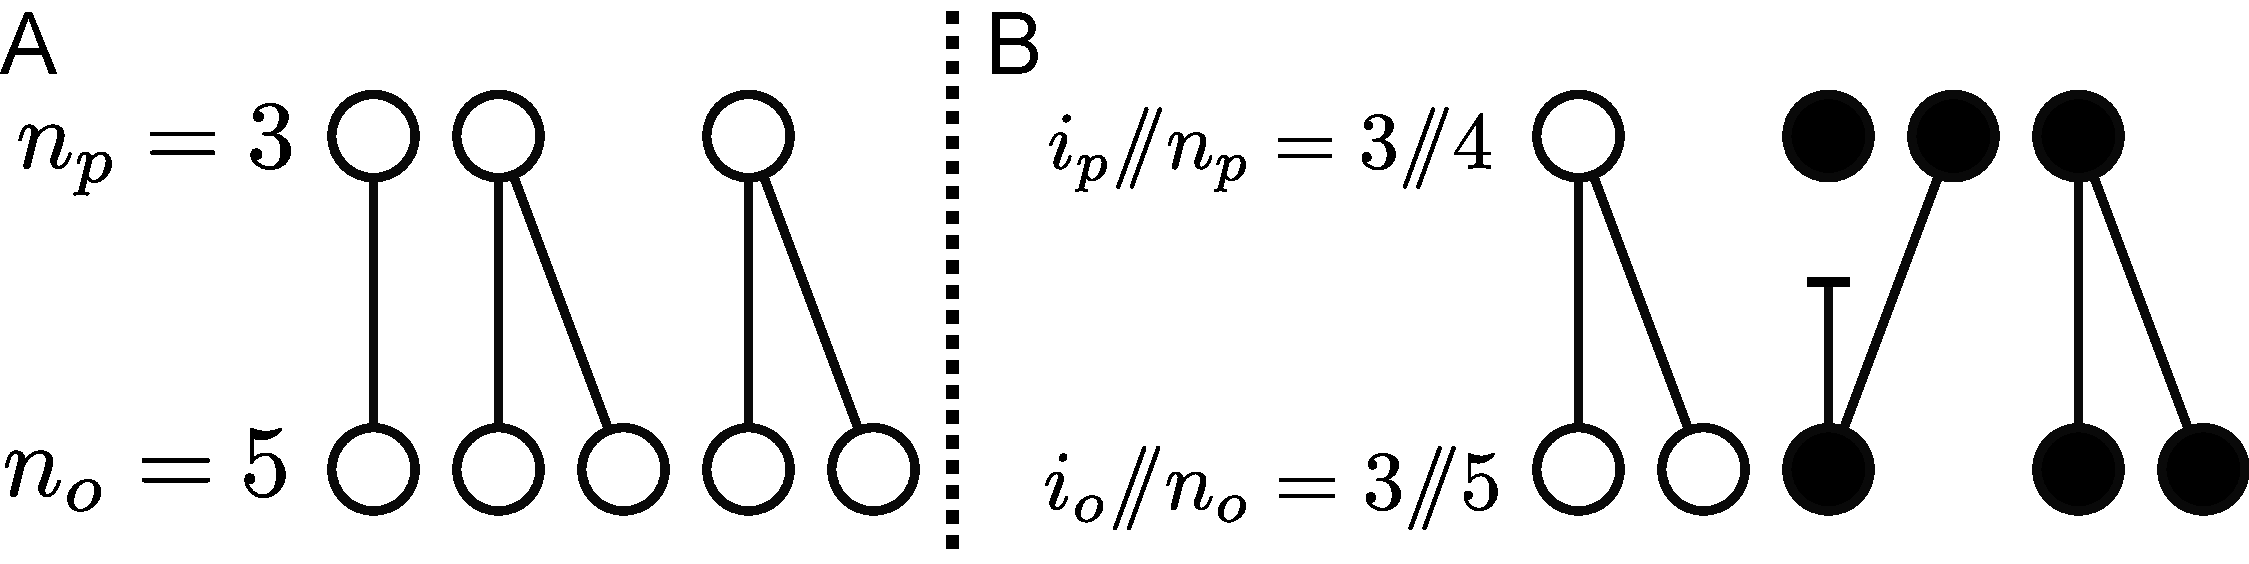
\includegraphics[width=1.0\columnwidth]{fig/schematic-AB.pdf}

  \caption{\label{fig_schematic}
    Realizations of sampling parental lineages under neutrality (A) and under selection (B). The top
    and bottom rows respectively represent the $n_p$ parents and $n_o$ offspring. Filled circles
    indicate the $i_p$, or $i_o$ copies of the derived allele; empty circles are ancestral alleles.
    A line connecting two circles represents a successful draw, a broken line - a selective death
    triggering a redraw.  }

\end{figure}


To express the allele-frequency spectrum $\afsPsi{n_o}{t}(i_o)$ for $n_o$ offspring in terms of the parental
\textit{AFS} at $t-1$, we can sum over possible values for random variables $n_p$ and the number $i_p$ of distinct derived alleles
among the parents:
\begin{equation}
  \afsPsi{n_o}{t}(i_o)=\sum_{n_p,i_p} P_{n_o}(i_o,i_p,n_p),
\end{equation}
where the subscript $n_o$ indicates dependence on parameter $n_o$. 



To obtain a recursion on the
\textit{AFS}, we use an exchangeability property of the parental lineages. Since the order in which we
draw new parental lineages in the Wright-Fisher model is random, we can first draw a random permutation 
of the parental population, and then select unsampled parents in order from this permutation. 
This allows us to separate properties of this permutation,
which depend only on parental \textit{AFS}, from properties of Wright-Fisher sampling, which depend
on population size and selection coefficients. Concretely, the event $(i_o,i_p,n_p)$ that we draw
$i_o$ derived offspring alleles from $n_p$ distinct parents of which $i_p$ are derived can be
expressed as the intersection of two events, $\mathcal{C}(i_p,n_p)$ and $\mathcal{S}_{n_o}(i_o,
n_p)$. Event $\mathcal{C}(i_p,n_p)$ specifies that the first $n_p$ parental lineages from the random
permutation carry $i_p$ derived alleles. Event $\mathcal{S}_{n_o}(i_o, n_p)$ requires that the
Wright-Fisher drawing process of $n_o$ offspring drew $i_o$ derived offspring alleles and sampled
exactly $n_p$ distinct parental lineages. Event $\mathcal{C}(i_p, n_p)$ depends on the allele
frequency distribution in the parental generation: $P(\mathcal{C}(i_p,n_p)) =\afs{n_p}{t-1} (i_p)$ by
definition of the \textit{AFS}. Thus
\begin{equation}
  \begin{split}
    \afsPsi{n_o}{t}(i_o)&= \sum_{n_p,i_p} P_{n_o}(\mathcal{S}_{n_o}(i_o, n_p), \mathcal{C}(i_p,n_p) )\\
    &=   \sum_{n_p,i_p} P_{n_o}(\mathcal{S}_{n_o}(i_o, n_p)| \mathcal{C}(i_p,n_p) ) P(\mathcal{C}(i_p,n_p))\\
    &=   \sum_{n_p,i_p} P_{n_o}(\mathcal{S}_{n_o}(i_o, n_p)| \mathcal{C}(i_p,n_p) )  \afs{n_p}{t-1}(i_p)%\\
%    \afs{n_o}{t} &\equiv  \sum_{n_p}  \mathbf{T}_{n_o,n_p}     \afs{n_p}{t-1}.
  \end{split}
\end{equation}
Using matrix notation to account for the sum over $j_o$ and $i_p,$ we have
\begin{equation}
  \afs{n_o}{t} = \mathbf{M}  \afsPsi{n_o}{t} =  \mathbf{M}  \sum_{n_p}  \mathbf{T}_{n_o,n_p}     \afs{n_p}{t-1}
    \label{eq_recur}
  \end{equation}
where $\mathbf{T}_{n_o,n_p}(i_o,i_p) = P_{n_o}(\mathcal{S}_{n_o}(i_o, n_p)| \mathcal{C}(i_p,n_p) ) $ 
can be thought of as $(n_o+1) \times (n_p+1)$ transition
probability matrix, whose row and column indices correspond to the number of derived alleles in the
offspring and contributing parental lineages, respectively. $\mathbf{M}$ is an $n_o\times n_o$ matrix encoding the effects of mutation. Related recursions under general neutral 
models were studied in \cite{Lessard2010}.

The \textit{AFS}  $\afs{n_p}{t-1}$ for any  $n_p\leq n_o$ can be obtained by downsampling from $\afs{n_o}{t-1}$ (\textit{i.e.}, $\afs{n_p}{t-1} =
\mathbf{H}_{n_p,n_o} \afs{n_o}{t-1}$ for hypergeometric projection matrix $\mathbf{H}_{n_p,n_o}$ if
$n_p\leq n_o$). Thus, Equation \eqref{eq_recur} provides a closed form recursion for $\Phi_{n_o}$ under neutrality. 
This was used in \cite{JouganousEtAl2017} to efficiently 
compute distributions of allele frequencies under neutrality and in small sample sizes.

Under selection, $n_{p}$ may be larger than $n_o$, leading to a set of $N$ coupled equations that is
typically too large to solve numerically (in the diffusion limit, the number of coupled equations is
infinite). But if the number of drift events is typically larger than the number of selective
deaths, as happens in large sample sizes, the coupling is weak and we can restore approximate
closure by truncating the summation in Eq. \ref{eq_recur}:

\begin{equation}
\begin{split}
  \afsPsi{n_o}{t}(i_o)
  &= \sum_{n_p=1}^{n_{o}} \mathbf{T}_{n_o,n_p}  \afs{n_p}{t-1}+ \sum_{n_p> n_o }  \mathbf{T}_{n_o,n_p} \afs{n_p}{t-1} \\
  &=      \sum_{n_p=1}^{n_{o}} \mathbf{T}_{n_o,n_p} \mathbf{H}_{n_p,n_o} \afs{n_o}{t-1}+ \sum_{n_p> n_o }  \mathbf{T}_{n_o,n_p} \afs{n_p}{t-1} \\
  &\equiv \mathbf{Q}_{n_o}                                               \afs{n_o}{t-1}+ \epsilon
\end{split}
\label{eq_truncated}
\end{equation}
where $\mathbf{Q}_{n_o} =  \sum_{n_p=1}^{n_{o}} \mathbf{T}_{n_o,n_p} \mathbf{H}_{n_p,n_o}$ is a
square matrix whose $(i_p,i_o)^\text{th}$ element is the probability $P_{n_o}(\mathcal{S}_{\leq n_o}
(i_o)| \mathcal{C}(i_p,n_p))$ of event $\ms_{\leq n_o}(i_o)$ that we observe $i_o$ derived alleles
in a sample of size $n_o$ and that we draw \emph{at most} $n_o$ distinct parental lineages (see
Appendix \ref{subsec_apx_tpm_deriv}), given event $\mathcal{C}(i_p,n_p)$ that $i_p$ of the first
$n_p$ parental alleles are derived.  

The term $\epsilon \equiv \sum_{n_p> n_o }  \mathbf{T}_{n_o,n_p} \afs{n_p}{t-1} $ 
accounts for events with $n_p>n_o.$ We will show below that it is small and often 
negligible for large sample sizes \sgcomment{Point to figure/result, or remove this statement. }. 
Further, it can be estimated to ensure convergence even in moderate sample sizes.  
Using the jackknife extrapolation of \citep{Gravel2016}, we can write  
$\afs{n_p}{t-1} \simeq J_{n_p,n_o} \afs{n_o}{t-1},$ where $J_{n_p,n_o}$ is a $n_p\times n_o$
matrix obtained by jackknife extrapolation, and thus
\begin{equation}
  \afsPsi{n_o}{t}(i_o) \simeq \tilde{\mathbf{Q}}_{n_o}        \afs{n_o}{t-1}
\label{eq_truncated_jack}
\end{equation}
with  $ \tilde{\mathbf{Q}}_{n_o} =  \mathbf{Q}_{n_o}  +   \sum_{n_p=n_o+1 }^{n_o+\delta}  \mathbf{T}_{n_o,n_p} J_{n_p,n_o}$
and $\delta$ is a parameter describing the order of the jackknife approximation to consider. 

Jackknife approaches have been used in \cite{JouganousEtAl2017} to derive approximate 
recursion equations under weak selection. But whereas the approach of \cite{JouganousEtAl2017} 
requires a jackknife approximation to create a new lineage for every selective death, the formulation in Equation \eqref{eq_truncated}
only requires approximations in the (rare) instances where there are more selective deaths than 
common ancestry events. By accounting for simultaneous events, lineages that go unused due to genetic drift can be repurposed to model selection (Figure \ref{fig_schematic}b).
Thus by keeping track of simultaneous events in the transition matrices
in \eqref{eq_recur}, we can drastically reduce our reliance on approximations.

Our next goal is to compute these matrices.

\section{Methods and Results}
\label{sec_methods}

\subsection{Constructing the transition matrix}
\label{subsec_trans_mat}

Even though $\mathbf{T}_{n_o,n_p}$ in Equation \ref{eq_recur} is a combinatorial probability
describing a single generation in the Wright-Fisher model, we were unable to compute an analytical
expression for it, while simultaneously allowing for multiple coalescences and multiple selective events.
However,
we can obtain fairly simple recursion by conditioning on the last draw. Such recursions were used for
describing large sample size effects without selection in \citep{BhaskarEtAl2014}. In this section,
we provide some mathematical intuition, and a more detailed derivation is provided in the
Appendix \ref{subsec_apx_tpm_deriv}.

Under selection, the last draw can be characterized by whether it was successful or rejected,
whether it drew a derived or ancestral allele, and whether it drew a previously drawn parental
lineage or not (Figure \ref{fig_rec_selection_dynamic_fail}).  The state of the sampling process
prior to the last draw can be described by a number of successfully drawn offspring $n'_o$, of which
$i'_o$ are derived, a number of distinct parental lineages $n'_p$ of which $i'_p$ are derived, and a
number of failures since last successful draw $r'$.  The recursion will be over a probability
$\mathbf{T}_{r}\Coalc{i_p}{n_p}{i_o}{n_o}$ which generalize the transition matrices from Equation
\eqref{eq_truncated} to account for rejected draws: $\mathbf{T}_{n_o,n_p}\equiv
\mathbf{T}_{r=0}\Coalc{i_p}{n_p}{i_o}{n_o}$. Formally,  $\mathbf{T}_{r}\Coalc{i_p}{n_p}{i_o}{n_o}
\equiv P_{n_o}\left[\ms_{n_o}(i_o, n_p, r) | \mathcal{C}(i_p, n_p)\right]$ where $\ms_{n_o}(i_o,
n_p, r)$ is a generalization of  $\ms_{n_o}(i_o, n_p)$ that accounts for rejected draws: it is the
event that $i_o$ of the first $n_o$ successfully drawn offspring are derived, that the following $r$
draws are rejected, and that the $n_o$ offspring and subsequent $r$ failures required exactly $n_p$
distinct parental draws.  The bracket notation, $\mathbf{T}_{r}\Coalc{i_p}{n_p}{i_o}{n_o}$, is
convenient to keep track of the number of relevant parental lineages (top of bracket) and offspring
lineages (bottom of bracket) in the recursion at the cost of obscuring their different probabilistic
role.

We show in the Appendix and illustrate in Figure \ref{fig_rec_selection_dynamic_fail}  that we
can express $\mathbf{T}_{r}\Coalc{i_p}{n_p}{i_o}{n_o}$ as a sum over a small number of terms
of the form $\mathbf{T}_{r'}\Coalc{i'_p}{n'_p}{i'_o}{n'_o}.$ If $r>0,$ the last draw must be a failure
and $r' = r - 1$ (leading to cases \textit{rC, rD} in Figure \ref{fig_rec_selection_dynamic_fail}).
If $r=0,$ the last draw must be a success and $n_o' = n_o-1$ (cases \textit{A} to \textit{D})

% Figure \ref{fig_rec_selection_dynamic_fail} shows a graphical representation of the recursion, and
%A mathematical derivation is provided in the appendix.
%The recursion can be broken down in a recursion over $r$, determined by rejected draws,
%and a recursion over $n_o$, determined by successful draws.
%The recursion over $r$ is shown at the bottom of
%Figure \ref{fig_rec_selection_dynamic_fail} (cases \textit{rC,rD}). If the last draw was rejected, the sampling
%prior to the last draw must have ended with $r-1$ rejected draws. We
%must simply track whether the last rejected draw was from a previously drawn parental lineage (case
%\textit{rD}), in which case the number of parental lineages is unchanged, or of a new lineage (case
%\textit{rC}), in which case the sample with $r-1$ rejections must have had exactly one fewer distinct parent and
%one fewer derived parental allele than the full sample.

%Thus we can obtain $\mathbf{T}_{r}\Coalc{i_p}{n_p}{i_o}{n_o}$ from
%$\mathbf{T}_{r-1}\Coalc{i_p-1}{n_p-1}{i_o}{n_o}$ and $\mathbf{T}_{r-1}\Coalc{i_p}{n_p}{i_o}{n_o},$
%and recursively back to terms of the form $\mathbf{T}_{0}\Coalc{i_p'}{n_p'}{i_o}{n_o}$, with $n_p'\leq n_p$

%To progress further and express $\mathbf{T}_{0}\Coalc{\cdot}{\cdot}{i_o}{n_o}$ in terms of
%$\mathbf{T}_{r}\Coalc{\cdot}{\cdot}{\cdot}{n_o-1}$, we condition on the last successful draw. This
%last successful draw can be (Figure \ref{fig_rec_selection_dynamic_fail}) previously unsampled
%derived (A), sampled derived (B), unsampled ancestral (C), or sampled ancestral (D).

A challenge with this recursion is that the number of rejected lineages $r$ leading to each successful
draw can be infinite, in principle.
 However, the probability of having $r$ selective deaths for a single successful draw decreases
rapidly with $r$, as $s^r.$ We therefore modify the Wright-Fisher model such that at most $r_{max}$ failed
draws \emph{per offspring} are allowed, after which the next draw is immune to selection. Given
$s<1$, we can easily pick $r_{max}$ to ensure excellent convergence. For example, with $s=0.01$,
which corresponds to $Ns=100$ with $N=10,000$, the probability of having more than
three selective deaths is less than $10^{-8}$, and the probability of having more than eight selective deaths is
less than $10^{-18}.$ We have used $r_{max}=3$ in numerical calculations presented below, but a 
more stringent cutoff does not present particular challenges.

Using caching to avoid re-computing previously computed values, we can systematically compute all the terms in Equation
\ref{fig_rec_selection_dynamic_fail}.
\begin{figure}
  \centering
  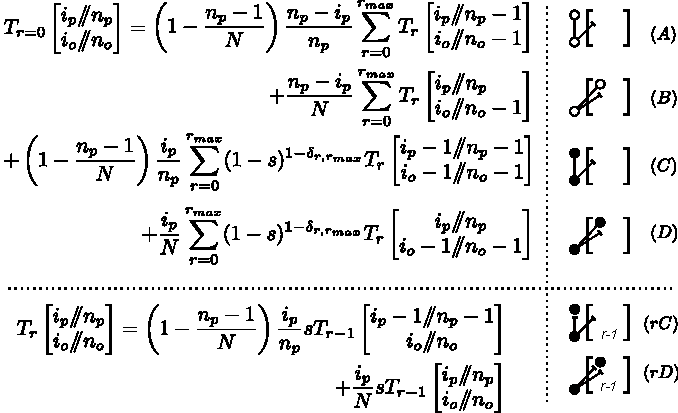
\includegraphics[angle=-90,width=1.1\columnwidth]{fig/recurrence-selection-dynamic-failures-annotated.pdf}

  \caption{Recursion over the last draw for transition probabilities with selection. 
    The right hand panel represents the last draw graphically.
    Filled and empty circles represent derived and ancestral alleles. 
    Solid and broken lines are
    successful lineage draws and re-draws due to selection.
    Square brackets represent events in sample of size $n'_o$ prior to the last draw. Summands
    (\textit{A-D}) are successful draws where the last lineage is ancestral (\textit{A,B}) or
    derived (\textit{C,D}). A successful draw can happen after
    $0$ to $r_{max}$ failed draws, which is accounted for by the sum in the recursion . Terms \textit{rC} and \textit{rD}
    represent the probability that last draw was rejected. See Table \ref{tab_symbols} for notation used.
  }

  \label{fig_rec_selection_dynamic_fail}
\end{figure}
The set of selection transition probability matrices $\mathbf{T}$ requires $O(r_{max}n_o^2 n_p^2)$
operations to construct: Since each entry in $\mathbf{T}_{r}$ (with $r>0$)  in the recursion requires a
constant number of operations, the computational complexity depends on the number of terms we need
to calculate. We will need to compute terms of the form
$\mathbf{T}_{r}\Coalc{i_p'}{n_p'}{i_o'}{n_o'}$, with $1 \leq n_o'<n_o$, $i_o' \leq n_o'$, and $0\leq
i_p' \leq n_p' \leq n_p$, and $0\leq r \leq r_{max},$ leading to the bound $O(r_{max}n_o^2 n_p^2).$

The terms  $\mathbf{T}_{r=0}$ have a bound of the same form (i.e., there are at most $O(n_o^2 n_p^2)$
terms, each requiring $r_{max}$ computations).  Finally, the truncated matrix $\mathbf{Q}_{n_o} =
\sum_{n_p=1}^{n_{o}} \mathbf{T}_{n_o,n_p} \mathbf{H}_{n_p,n_o}$ can be constructed in $O(n_o^4)$.

This is moderately more complex than in the neutral case, where recursions \citep{BhaskarEtAl2014}
 and analytical expressions \citep{Lessard2010} can be computed in $O(n_o^3).$


\subsection{Calculation of allele frequency spectra}
\label{subsec_afs}

Once the truncated matrix $\mathbf{Q}_{n_o}$ from Eq. \ref{eq_truncated} or 
the jackknife-corrected  $\tilde {\mathbf{Q}}_{n_o}$ are constructed, they can be
used to calculate the allele frequency spectrum under a wide range of models \citep{JouganousEtAl2017}. 
To validate the method, we estimate the equilibrium
distribution where exact solutions are available \citep{Krukov2016}. In the infinite sites model at
equilibrium, we can compute the equilibrium \textit{AFS}, $\Phi$ in a finite sample as a solution to
a linear system:
\begin{equation}
  \label{eq_sfs_calc}
  \Phi = \mathbf{Q}\Phi  + n \mu e_1
\end{equation}
where $\mu$ is the per-site (forward) mutation rate and $e_1$ is the second column of the identity
matrix of size $n+1.$ Since the infinite-sites model does not account for fixed sites,
we only report frequency spectra for polymorphic sites below.

Figure \ref{fig_strong_selection} shows the comparison of the \textit{AFS} calculated from Equation
\ref{eq_sfs_calc} with a jackknife of order 5,
the diffusion approximation \cite[eq. 9.23]{Ewens2004}, and the numerical
calculation performed in \texttt{moments} \citep{JouganousEtAl2017}. In all the panels, the sample
size is $n=200$ individuals. Any allele frequency probabilities below $1\times10^{-12}$ are not
included in the figures. 

\textit{AFS} computed using the recursion with the jackknife (Figure \ref{fig_strong_selection}) are 
indistinguishable from the exact Wright-Fisher solution \textit{AFS} in all the examined 
parameter ranges. \textit{AFS} computed using the present approach without the jackknife 
(i.e., with pure truncation, $\epsilon = 0$, Figure \ref{fig_apx_no_jackknife}) show moderate departures from the exact results, 
mostly at high allele frequencies where the number of observations is low. 
Distributions of allele frequencies using \texttt{moments} with a jackknife shows 
excellent agreement to predictions of the diffusion approximation for small selection 
coefficients, but visible discrepancies with $Ns\ge 50.$ Thus selection is treated more 
accurately in the present approach, as expected. 


However, the larger difference between the two approaches stems not from the difference in the accuracy of the jackknife approximations but in the
contrast between diffusion-based and Wright-Fisher-based genealogies.

Figures \ref{fig_strong_selection}A,B show that there is a disagreement between the exact
Wright-Fisher and the diffusion solutions for singletons, doubletons, and $(n-1)$-tons even under neutrality. 
This effect increases with sample size, and has been observed by comparing
Kingman's coalescent with multiple-merger coalescent events in \citep{Fu2006, BhaskarEtAl2014}.


%Figures \ref{fig_strong_selection}B,D show the special case where the sample is the entire
%population, where the large sample effects are maximized. Note the difference in the $X$-axes for
%these panels.

Figures \ref{fig_strong_selection}C,D show a comparison at moderate negative selection, $Ns=10$.
Here, we see a stronger difference between diffusion and Wright-Fisher models. 
Comparisons under more parameter choices can be found in  Figure~\ref{fig_apx_strong_selection_extended}.

\begin{figure}
  \centering
  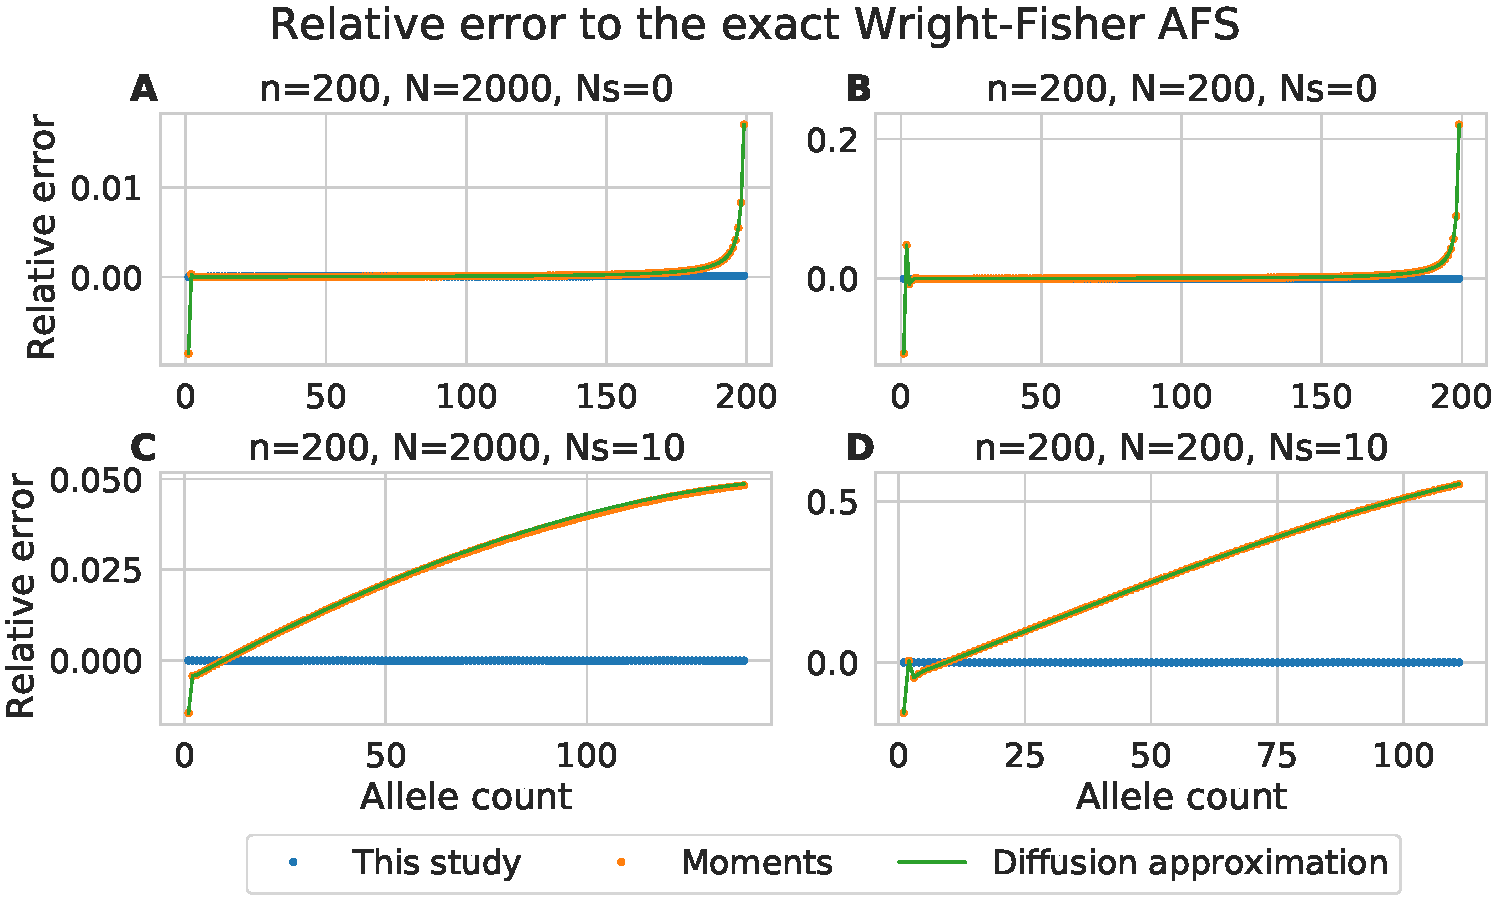
\includegraphics[width=\columnwidth]{fig/afs_comp_small.pdf}

  \caption{Relative error of allele frequency spectra in a sample of size $n=200$ with respect to
    the Wright-Fisher model. Neutral ($Ns$=0) (A,B), or deleterious alleles ($Ns=10$) (C,D). (A) shows
    the frequency spectrum in a sample from a large population ($N=2000$), (B) The sample is entire
    population ($n=N=200$). At neutrality all the models agree, except at high allele frequencies.
    With negative selection, the predictions differ substantially at moderate allele frequencies.
    Note that $Y$-axes are at different scales between the panels. An extended version of the figure
    is shown in the appendix - figure \ref{fig_apx_strong_selection_extended}.}

  \label{fig_strong_selection}
\end{figure}

Because differences between diffusion and Wright-Fisher models are tied to multiple merger events, 
we do not expect large differences in quantities such as the genetic load, and this is confirmed
in Supplementary Table \ref{tab_apx_load}. 
Rather, the distribution of allele frequencies in Figure \ref{fig_strong_selection}
 indicates that a higher proportion of the load is caused by common variants  
 under the diffusion model relative to the Wright-Fisher model. 

This excess of high-frequency deleterious variants in diffusion models suggests a difference 
in the rates of fixation of deleterious alleles. 
Figures \ref{fig_apx_fixation_100} and \ref{fig_apx_fixation_1000} show that these differences 
remain modest except for fairly deleterious alleles and small populations,
where the differences are large enough to affect mean fitness over evolutionary time-scales. 


When the sample is the entire population, as in figures \ref{fig_strong_selection} B and D, the
present method is exact. It is also not needed, since exact recursion equations can be obtained 
from binomial sampling (\textit{i.e.}, there is no computational benefit to consider a subsample that is as
large as the entire population).  The present approach is useful where accurate recursions can be
obtained for sample sizes that are appreciably smaller than $N$. We therefore seek asymptotic
results for the convergence of the recursion approach in the following sections.

\subsection{Estimating the missing probability}
\label{subsec_missing}

%Truncation in equation \ref{eq_truncated} means that if $n_p > n_o$, some probability will be lost.

Given that $ \mathbf{Q}_{n_o}(i_p, i_o) = P_{n_o}(\mathcal{S}_{\leq n_o} (i_o)|
\mathcal{C}(i_p,n_p)),$ we can compute the fraction of unaccounted-for or approximated draws 
due to truncation:
Given $i_p$ derived among the first $n_o$ parental alleles, this is $1-\sum_{i_o} \mathbf{Q}_{n_o}(i_p,
i_o).$ From a numerical perspective, this allows for easy tracking of the proportion of the probability
transition that required a jackknife approximation. 
Figure \ref{fig_apx_missing} shows the probability of missing lineages under the worst-case
scenario where all parental alleles are derived, $i_p = n_p.$ 
The probability first increases with increasing sample size, as the number of draws that
can result in selective deaths increases linearly. However, the number of drift events eventually overtakes
the number of selective events, and the probability that we need additional lineages decreases
rapidly with sample size. Creating additional lineages via the jackknife approximation improves the performance further.

Supplementary section \ref{parent_distribution} provides analytical expressions for the probability distribution
$P(n_p-n_o) $ under worst-case scenario $i_p = n_p,$ as well as its
mean and variance. In particular, we show that
\begin{equation}
    \label{eq_lineages_approx}
    \hat{E}[n_p-n_o | n_o] \approx n_o  s - \frac{n_o (n_o-1) }{2N}.
\end{equation}

We thus have the usual interplay of selection and drift. Solving for $ \hat{E}[n_p -n_o | n_o]\leq0$
yields a critical sample size $n^*_o$ where there are more drift events than selection events in
the sample,

\begin{equation}
  \label{eq_critical_sample}
  n_o^* \ge 2N s.
\end{equation}

We also show that, to leading order in $s,$ $n_o/N,$ and $1/N,$ the variance is

\begin{equation}
  \begin{aligned}
    \operatorname{Var}[n_p-n_o | n_o] &\simeq
   n_o  s +   n_o (n_o-1)/(2 N).
    \label{eq_gauss_var}
  \end{aligned}
\end{equation}

Thus the mean and variance to leading order are those of the Skellam distribution: the
\textit{increase} in lineages can be modelled, to lowest order, as the number of lineages gained
through selection (modelled as Poisson with mean  $ n_o s$) minus the number of lineages lost to
drift (modelled as an independent Poisson variable with mean  $ n_o (n_o-1)/(2 N)$).
As the number of drift and selection events get larger, the Skellam distribution can be approximated as a
Gaussian with corresponding mean and variance.

%\begin{equation}
 % P(n_p|n_o) \sim \mathcal{N}(\mu, \sigma).
%  \label{eq_gaussian}
%\end{equation}

Figure \ref{fig_combined}A shows the excellent agreement between the exact distribution and the
Gaussian approximation (using the exact variance from Equation \ref{eq_exact_var}). By contrast,
we don't expect this approximation to work well if the sample size is so small that few drift
events occur at a given generation, (say, $\frac{{n_o}^2}{2N} < 10$), where the Skellam
distribution is a better fit - Figure \ref{fig_apx_skellam}.

The Gaussian approximation using leading order terms provides intuition about regimes where we
expect drift to almost always overtake selection.  Appendix \ref{subsec_apx_gauss} shows that the sample size
$n_z$ required such that the expected loss in the number of lineages is $z$ times its standard deviation
obeys

\begin{equation}
  n_z \lessapprox 2 \sqrt{N} z + 2N s.
\label{eq_nz}
\end{equation}

The second term
encodes the condition that there are more coalescence events than selection events, on average. 
It is comparable to contemporary sample sizes even under strong selection (say, $2Ns=100$).
The
first term is independent of $s$ and can be interpreted as a condition that there are sufficient
drift events per generation to ensure that the probability of having zero drift event is weak: $n_z
= 2 \sqrt N z$ implies $\frac{n_z^2}{2N}= 2 z$. One interpretation is that we need at least a few
expected coalescence events per generation to ensure that every selective event is compensated by a
coalescence event at the same generation.

%Alternatively, we can solve for the quantiles of the Gaussian approximation (eq. \ref{eq_gaussian})
%numerically.
 For a fixed $z=3$, Figure \ref{fig_combined}B shows the critical sample size relative to the population size
 $(n_c/N)$. Together with equation \ref{eq_nz}, this shows
that the truncation can be accurate even for strong selection and sample sizes much smaller than
the full population size.

If we extrapolate the Poisson model of the drift vs selection interplay in equations \eqref{eq_lineages_approx} and \eqref{eq_gauss_var},
we can approximate the critical sample size for a given parental frequency $x_p$ as
\begin{equation*}
  n_z \leq 2 \sqrt{N} z + 2Nsx_p,
\end{equation*}
suggesting that even very strong selection will not overcome drift even in moderate sample sizes. 

Thus a determinant of the accuracy of the present approach is not whether selection
is weak enough, but whether there is enough drift in our sample to ensure that each 
selection event is met by a drift event in the same generation. 

\subsection{Integrating over several generations}
This naturally suggests an improvement: if we consider transitions in the 
\textit{AFS}  not from one generation to the next, but from one generation to $g$ generations down the line, drift at one generation can compensate for selection events at another.  If the $n_o$ offspring depend on $n_p=n_o+1$ distinct parental lineages, because a selective event occurred, but these parental alleles depend on only $n_{gp} = n_o$ grand-parental lineages, because of a drift event, a transition matrix from the grand-parental AFS to the offspring AFS would be closed.   

Such a transition matrix require additional bookkeeping, summing over possible intermediate parental configurations. As it turns out, computing accurate transition matrices over a few generations is reasonably straightforward and not significantly more costly than computing single-generation matrices
(Appendix \ref{subsec_apx_multi}). If the expectation of $n_p-n_o \simeq n_o  s - \frac{n_o (n_o-1) }{2N}$ is negative, the probability that we require more than $n_o$ ancestral lineages $g$ generations ago decreases with $g.$
To get an idea of the truncation behavior
for small number $g \ll N$ of generations, we can approximate the change  in the number
of lineages as we go back in time as a random walk with (approximately) constant mean and
variance. In this case, both the mean and variance will be scaled by a factor $g$ relative
to the single-generation case, and Equation \eqref{eq_nz} becomes:
\begin{equation}
  n_z \lessapprox 2 z\sqrt{N/g} + 2N s x_p.
\label{eq_nzg}
\end{equation}

For example, consider a population of size $N=10,000$ with strong selection
of $2Ns = 100.$ 
%corresponding to a fixation probability reduced by a factor $4\times 10^{-42}$ relative
%to the neutral expectation \cite{Kimura:1962um}. 
 If we set $z=5$ and $g=10,$ for example, to reach high accuracy even without a jackknife,
  we require a sample size of at most $ 400 = 0.04 N.$

As long as $n>2Ns x_p$, we can choose a number of generations to ensure that the probability of 
$n_p>n_o$ is small.

\section{Discussion}
\label{sec_conclusion}

%Classically, the coalescent considers models in the absence of natural selection. Since selection
%can increase the number of contributing lineages back in time, the coalescent can no longer be
%represented by trees, but instead acquires a graph structure. The ancestral selection graphs
%\citep{KroneNeuhauser1997} deal with this in the limit of large population size ($N$).

The diffusion approximation and Kingman's coalescent models differ from 
the Wright-Fisher model in that they do not account for possible simultaneous events. 
A common interpretation is that they are approximations to the 
`exact' Wright-Fisher process (e.g., \cite{Fu2006}). In this interpretation, the approach presented here 
provides an overall more accurate way of estimating distributions of allele frequencies for deleterious variants 
in large samples than state of the art diffusion-based \cite{Gutenkunst2009} or recursion-based \cite{Jouganous2017} approaches. 

Under neutrality, where differences across models have been studied extensively, the coalescent remains useful 
as an approximation even in rather large sample sizes \citep{Fu2006}, although quantitative inference 
can be affected in realistically large samples \citep{BhaskarEtAl2014}. 
Overall, we find that the same holds under selection in 
large populations and modest selection coefficients, with differences being exacerbated and 
reaching qualitative levels in small populations and large selection coefficients 
(Figures \ref{fig_strong_selection} and \ref{fig_apx_strong_selection_extended}). 
 
Whereas differences among neutral models were restricted to the extremes of the distribution, 
differences under selection span the entire distribution of allele frequencies (Figure \ref{fig_strong_selection}). 
Such discrepancies point to differences in the distribution of gene genealogies that go beyond 
details of whether coalescence events are simultaneous or sequential within a generation. 
\cite{Fu2006} proposed a rather detailed comparison of gene genealogies under both 
(neutral) models.
 
To directly compare how within-generation differences affect long-time gene genealogies, 
we consider a discretized version of Kingman's coalescent in which the times of 
all coalescence events are rounded up to the previous generation. 
This discretization turns Kingman's coalescent into a Cannings model that has simultaneous and 
multiple mergers, but whose gene genealogies have, up to rounding, the same distribution as in 
Kingman's coalescent. 

Figure \ref{sibships} shows a comparison of sibship sizes under discrete Kingman coalescent 
and Wright-Fisher model, in a sample equal to the population of size $n=N=100 000$. 
The discretized coalescent has slightly larger families overall,
 (i.e., the rate of coalescence is slightly higher, as has been observed e.g. in \cite{Fu2006}), but 
the differences in sibship sizes are not uniform: There are a few more sibships of size 1 and many more families of size above 4 
in a coalescent model, whereas there are more parents with 0, 2, or 3 offspring under Wright-Fisher. Under neutrality, 
the excess of single-child families with the coalescent leads to an excess of deep singleton lineages and thus $(n-1)$-tons,
as discussed in \cite{Fu2006}. The abundance of large families within the coalescent provides a higher probability for
 new mutations, including deleterious ones, to rapidly reach appreciable frequency in the populations.
 
 \begin{figure}
  \centering
  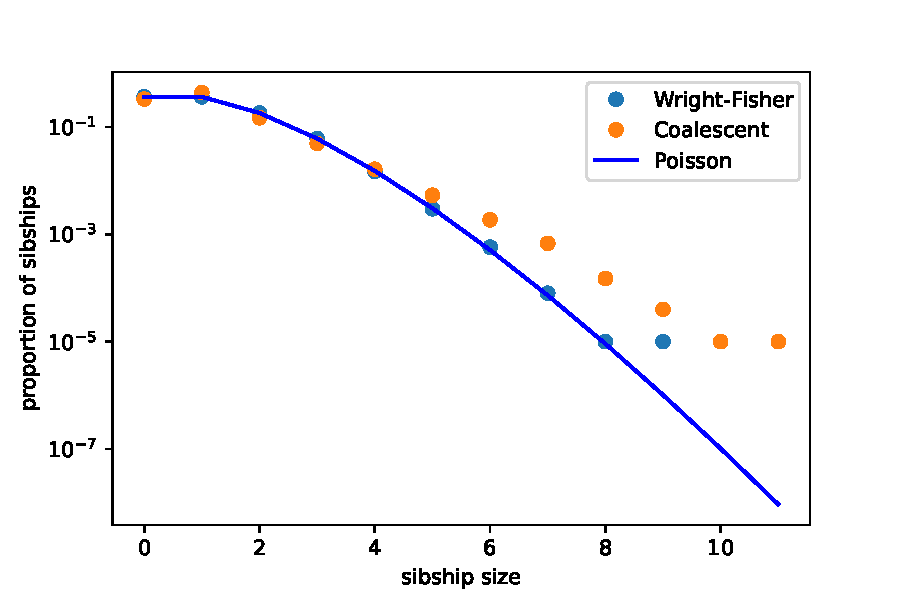
\includegraphics[width=\columnwidth]{fig/familysizes.pdf}

  \caption{Distribution of family sizes under Kingman's coalescent and Wright-Fisher model, as
     simulated under \texttt{msprime}.
  \cite{Nelson2020} in a population of size $100,000$. In Kingman's coalescent, the sibships with zero 
  siblings are obtained by computing $N-n_p.$ \label{sibships}. The solid line shows the Poisson distribution.}


\end{figure}
 
The larger differences in prediction of allele frequency distributions between Wright-Fisher and Kingman's 
coalescent models under selection is a bit of a concern for inference, as neither approach provides 
a particularly accurate model of the distribution of family sizes in real populations \sgcomment{cite something}.
If our inferences depend strongly on the differences between family sizes under the two models, 
we can expect that both models will perform poorly. 

As much as we would like to, we cannot state with confidence that recursions under the Wright-Fisher
model presented here are a more faithful representation of natural gene genealogies than those based on 
the coalescent. However, they do present substantial advantages. 

First, the handling of natural selection is more robust than in existing moments-based approach, as most selective
events are now treated exactly rather than using an empirically accurate but uncontrolled jackknife approximation. 

Second, the approach can be generalized to more robust models so that we are no longer bound to the diffusion approximation. 
\cite{Lessard2010} has derived recursions for a wide range of neutral models, and we expect that many of those,
including the ancestral selection graph, can be generalized to almost-closed recursions with selection. 

Finally, even though we focused here on simple demographies, many methods for the analysis of complex demographies, 
such as \texttt{momi} \citep{KammEtAl2017}, build on discrete transition matrices for the \textit{AFS} but have been limited to neutrality.
 The existence of robust transition matrices 
under selection opens up the possibility of extending these methods to handle natural selection.

A remaining challenge of the present approach is that the computation of the transition matrices is itself costly. 
It can be pre-computed, but this requires step-wise constant population sizes 
and selection coefficients. Efficient implementation of this approach for continuously-varying population
sizes and selection coefficients, in the style of the \texttt{moments} software, will require some additional analytical work.


%We have presented the current approach as an alternative to jackknife approximations in achieving
%moment closure. The two approaches are not mutually exclusive. Even though we have focused here on
%showing that approximate closure can be reached within a finite sample to high confidence by
%truncation, sampling instances that do not close can still be approximatively closed using jackknife
%approximations. Whereas the jackknife approach of \cite{JouganousEtAl2017} requires jackknifing a
%new lineage every time a selection event occurs, the approach presented here can be used to draw a
%new lineage only when drift fails to overcome selection (that is, only within small truncation term
%$\epsilon$ in Equation \eqref{eq_truncated}).

%The recursion equations themselves  are expressed in terms of combinatorial probabilities that can
%be computed recursively in polynomial time. These computations remain costly if transition matrices
%must be computed for time-dependent population sizes and selection coefficients. In such cases,
%series expansion of transition matrices in terms of $s$, $\frac{n_o}{N}$ and $\frac{1}{N}$ may be
%the most practical option.

%Here we have shown that setting the second term to zero can lead to asymptotically accurate computations.
%A jackknife approximation of the form $\afs{n_p}{t-1} \simeq J_{n_p, n_o} \afs{n_o}{t-1}$ for $n_p>n_o$ as in \cite{Gravel2016},
%would only require an approximation for the already small proportion of samplings that required $n_p>n_o.$


%Approximate closure of recursions requires the simulated sample size to be above a critical size of $2N_e s.$
%It is not uncommon to perform simulations of allele frequencies to model datasets with hundreds or
%thousands of samples \citep{Gravel:2011bg, Tennessen:2012ck}.
 %As argued in \citep{BhaskarEtAl2014},  this is a regime where diffusion-based approaches
 %struggle even under neutrality. We have shown that problems become even more severe under negative selection.

%  accurate simulations require accounting for multiple coalescence events.
% Conveniently, such simulations would also be in the regime where the present approaches would be accurate,
% meaning that selection can also be accounted for.


% relevant to present-day human samples.
%The probability that selective events are \emph{reliably} compensated by drift events, to the level of accuracy
%expected in most numerical approaches, is a more challenging requirement.
%Even if we chose to include drift over multiple generations, the present approach is relevant when
%$\sqrt{N}\lessapprox n \ll N$, that is, when the sample size is large enough that coalescences  are likely to
%occur at each generation, but small enough that focusing on the finite sample provides a useful speedup
%relative to modelling the entire population. As argued in \citep{BhaskarEtAl2014},  this is a parameter regime
% relevant to present-day human samples.

One of the main benefits of studying large sample sizes of whole-genome genetic data is to refine
our understanding of strongly deleterious variation \citep{karczewski2020mutational}. Performing
quantitative inference for such datasets will require models that can handle both strong selection
and large sample sizes.  Since the transition matrices defined here can be used in both forward
\citep{JouganousEtAl2017} and backward approaches \citep{KammEtAl2017}, they can help genetic models
catch up with the requirements of genetic data.

%Conveniently, we also showed that increasing the sample size has an unexpected beneficial consequence.
%As sample size increases, the number of distinct parents relevant to a sample becomes,
%with high probability, smaller than the sample itself. Even though this does not rescue
%all desirable properties of coalescent models, it means that recursion equations
%needed to calculate sample properties under complex demographic scenarios become nearly closed.

\section{Acknowledgements}
We thank Sabin Lessard and Aaron Ragsdale for useful discussions. 

\bibliography{taming-strong-selection}

\newcommand{\beginsupplement}{%
        \setcounter{table}{0}
        \renewcommand{\thetable}{S\arabic{table}}%
        \setcounter{figure}{0}
        \renewcommand{\thefigure}{S\arabic{figure}}%
        \setcounter{section}{0}
        \renewcommand{\thesection}{S\arabic{section}}%
     }
\beginsupplement
\section{Appendix}

\subsection{Additional figures}
\label{subsec_apx_figures}

\begin{figure}
  \centering
  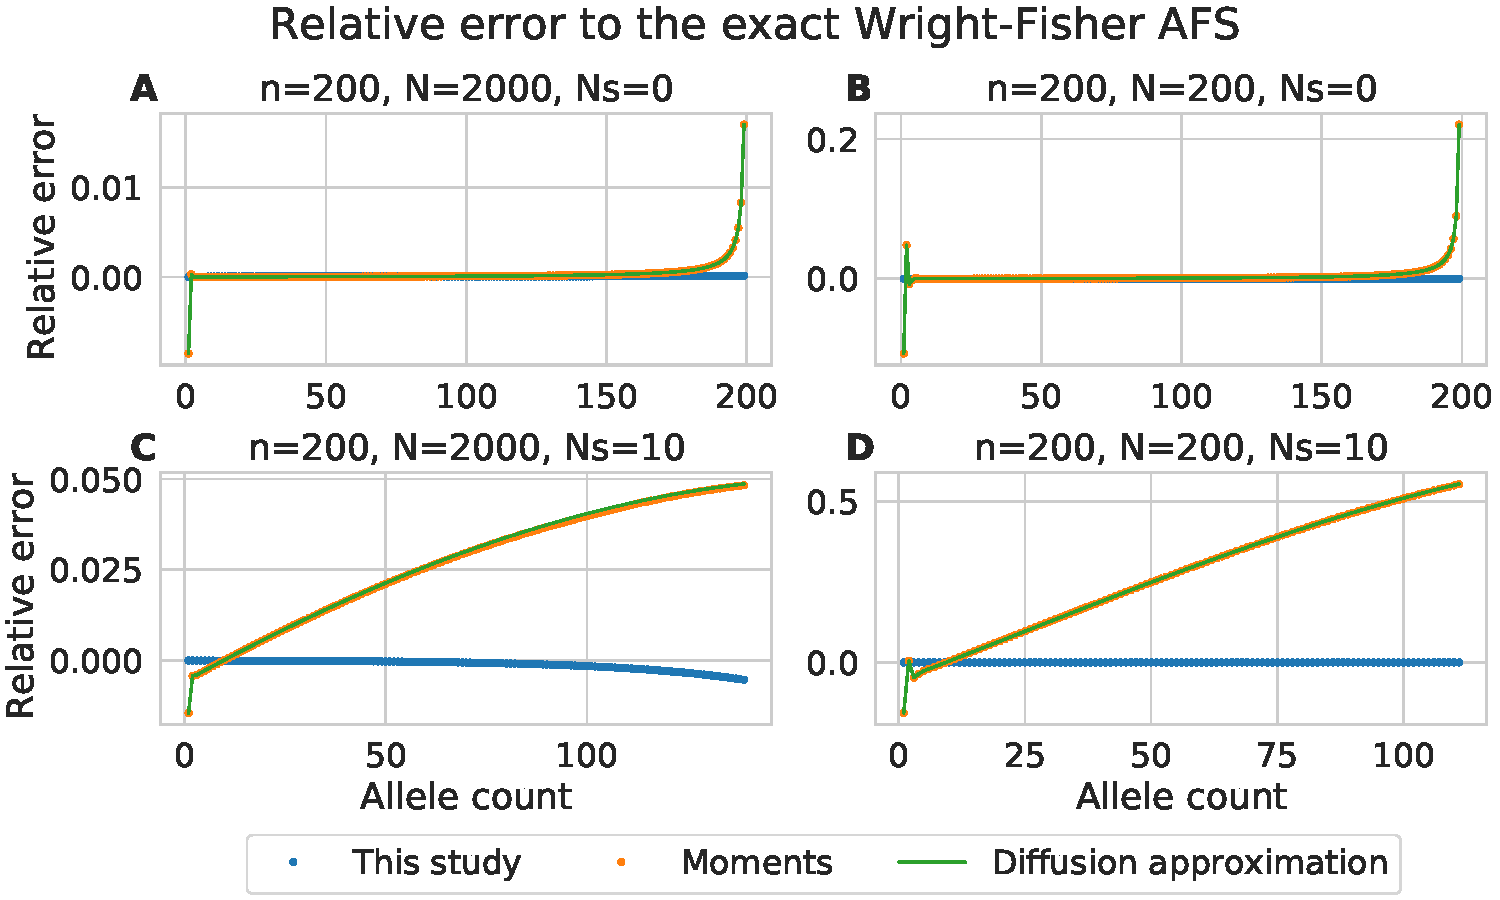
\includegraphics[width=\columnwidth]{fig/afs_comp_small_no_jackknife.pdf}

    \caption{Allele frequency spectra calculated in Figure \ref{fig_strong_selection} without the use of the jackknife.    }

  \label{fig_apx_no_jackknife}
\end{figure}

\begin{figure}
  \centering
  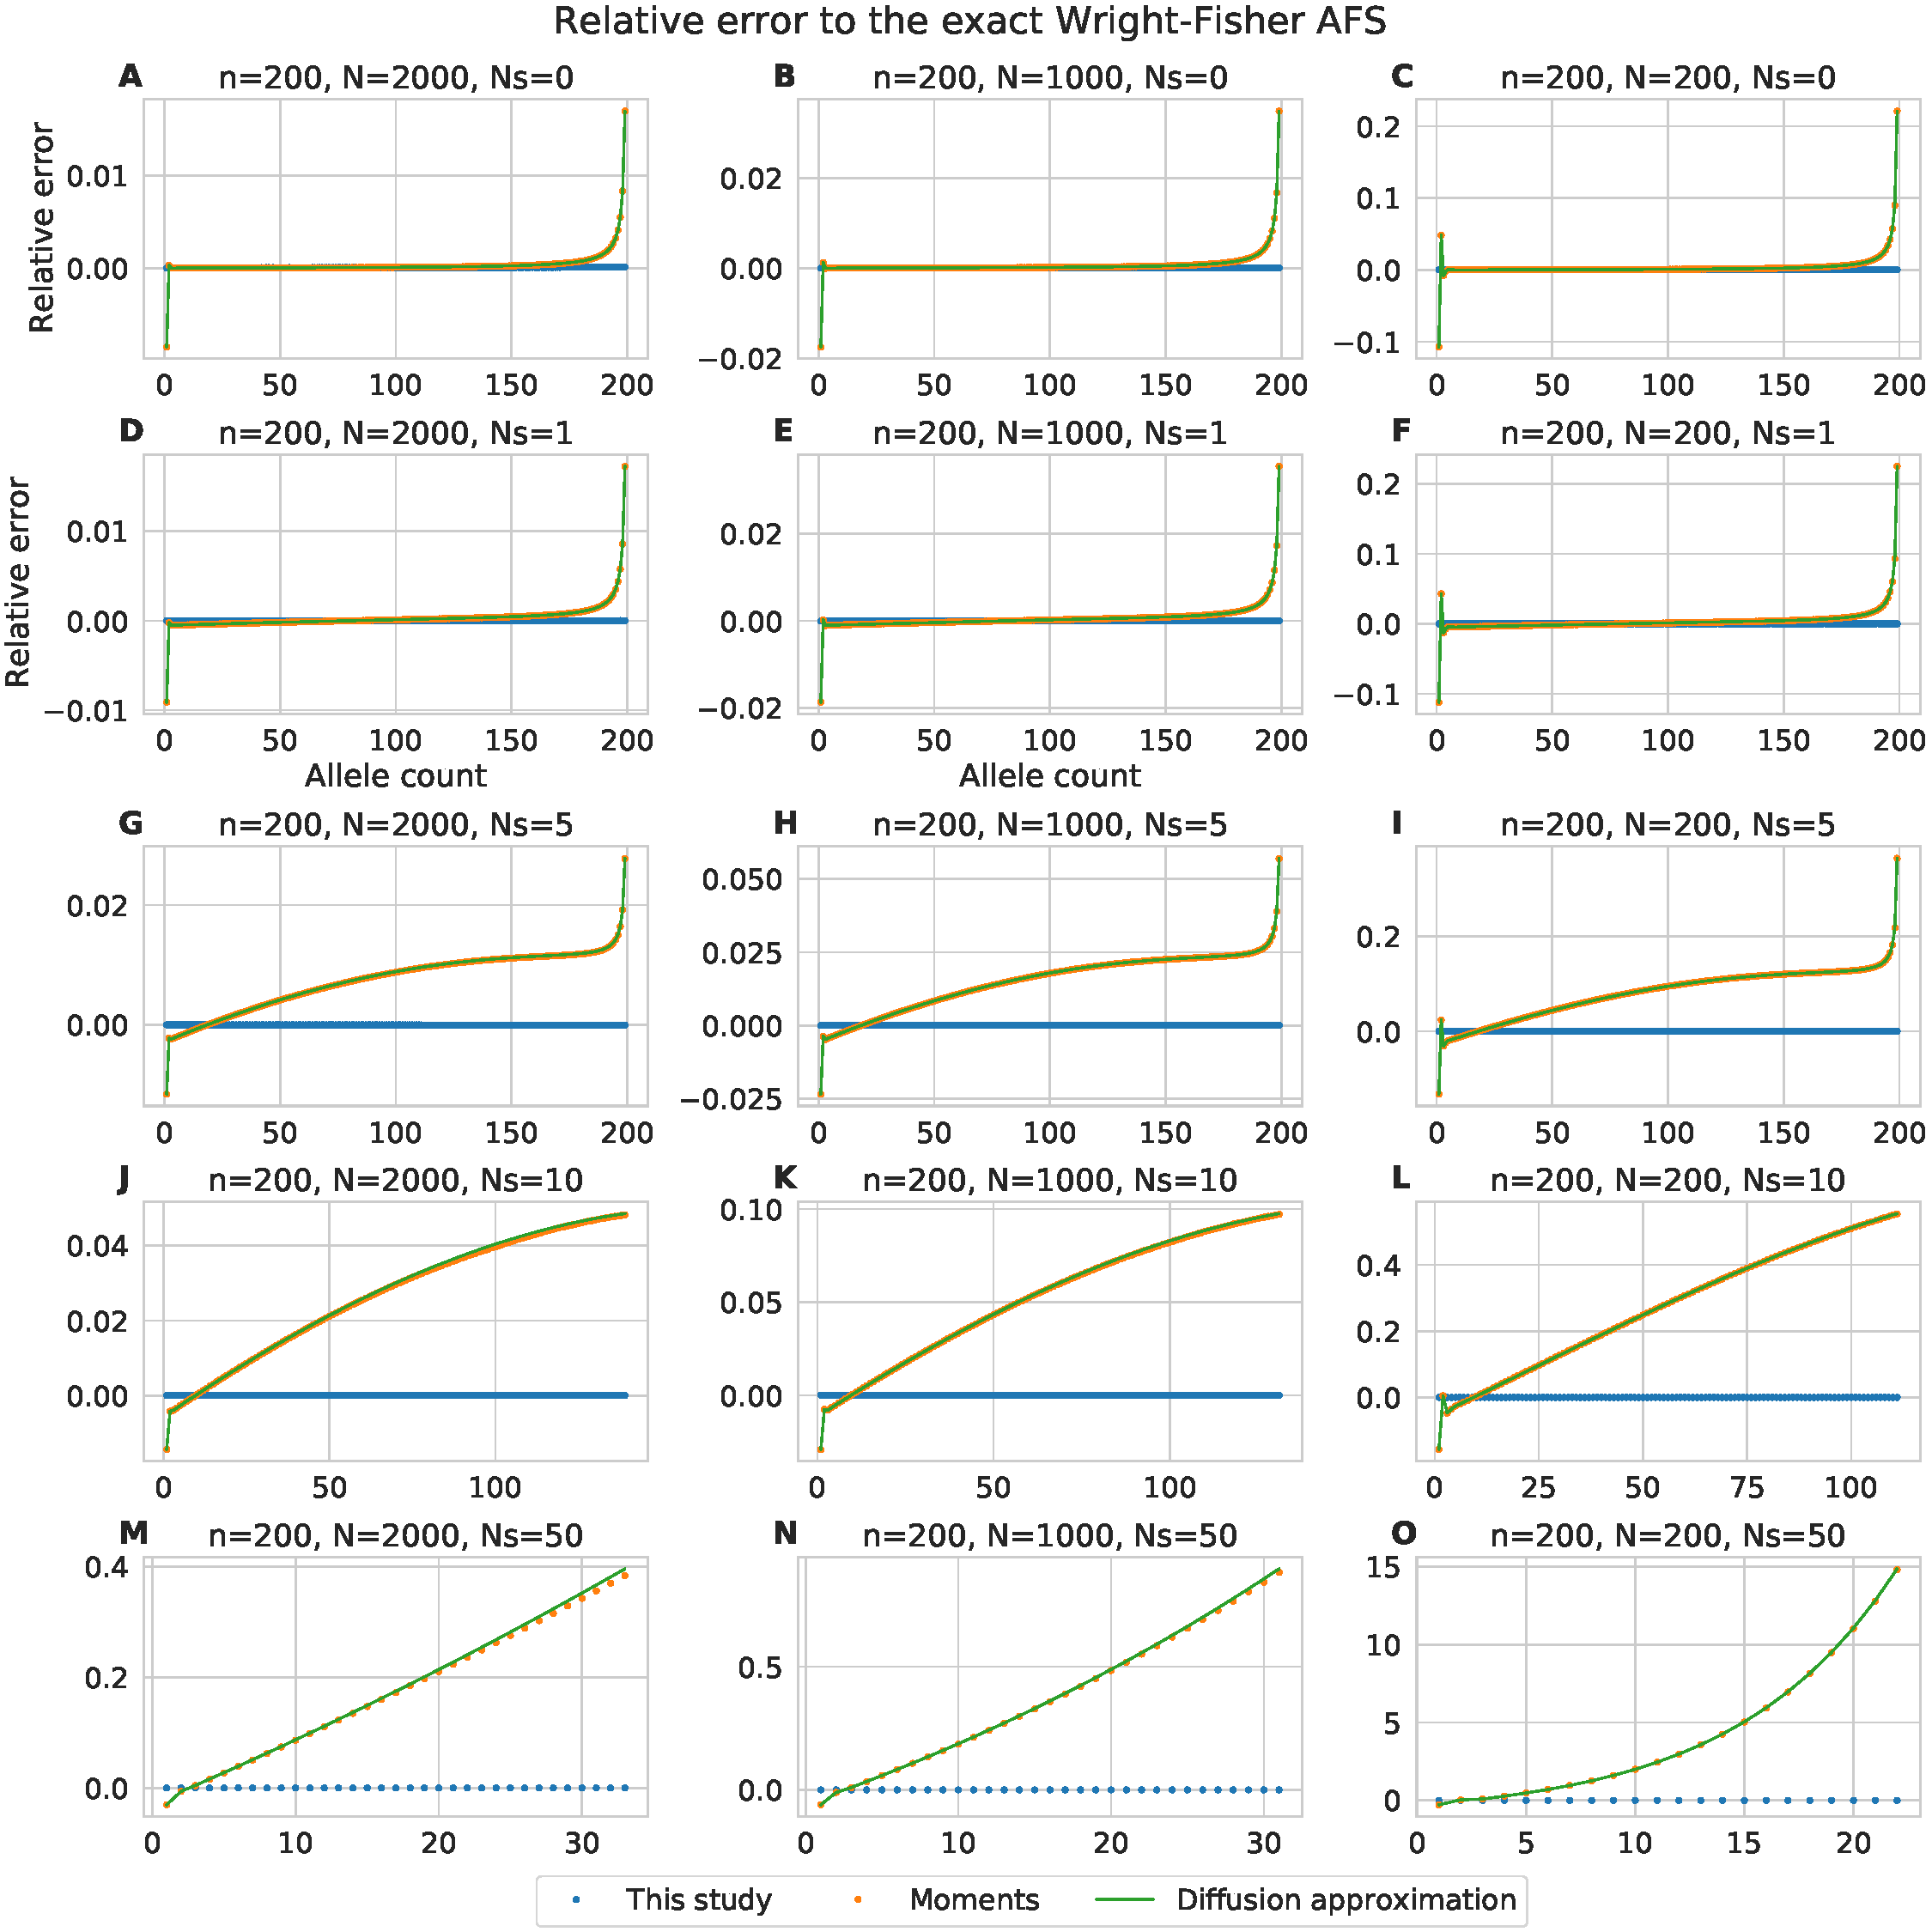
\includegraphics[width=\columnwidth]{fig/afs_comp_big.pdf}

    \caption{Extended version of figure \ref{fig_strong_selection}. Relative error of allele
    frequency spectra from different models with respect to the Wright-Fisher \textit{AFS}. Panels
    horizontally - population size ($N=2000,1000,200$). Note that the last column corresponds to the
    special case where the sample is an entire population. Panels vertically - selection
    coefficients ($Ns=0,1,5,10,50$). Note that in the strong selection case ($Ns=50$), the $X$-axis
    is truncated, such that the total probability of an allele at any frequency is above $1e-12$.
    }

  \label{fig_apx_strong_selection_extended}
\end{figure}

\begin{figure}
  \centering
  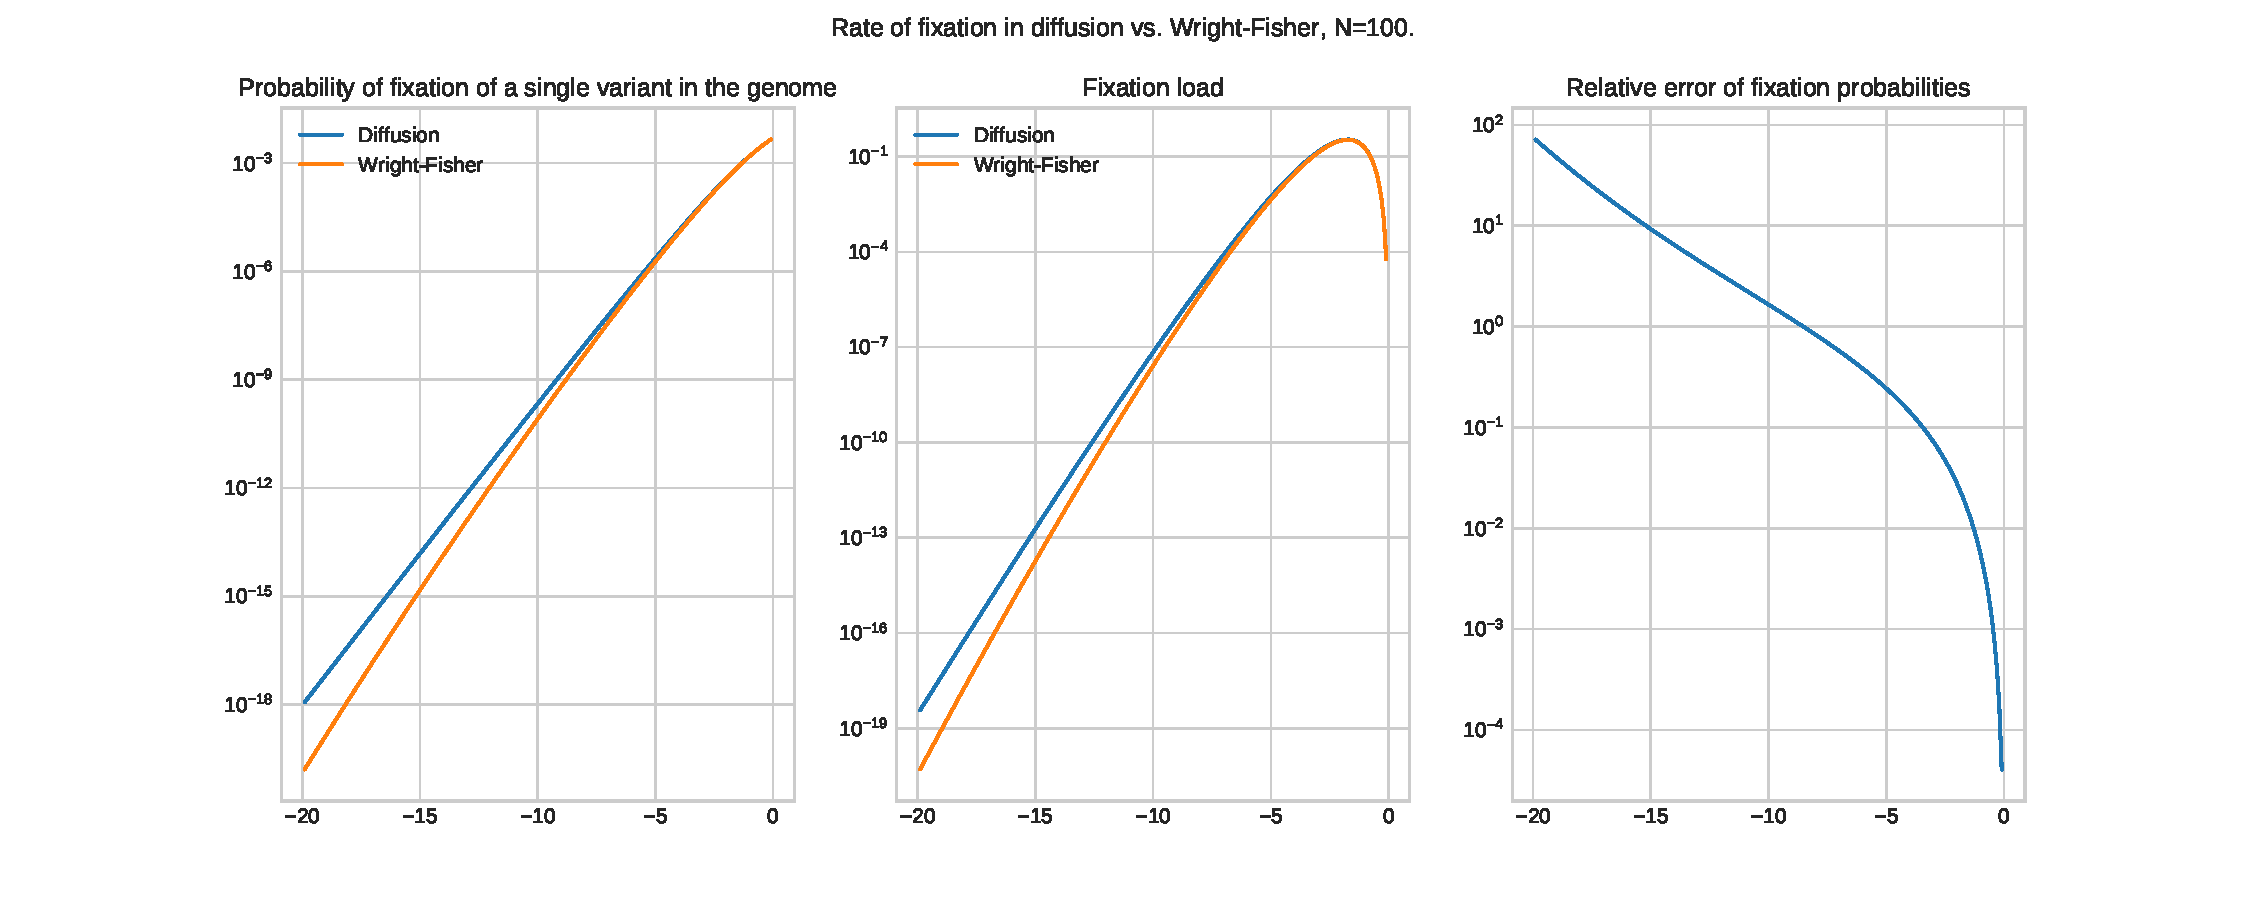
\includegraphics[width=\columnwidth]{fig/fixation_rate_N_100.pdf}

    \caption{(A) Fixation probability, (B) fixation load, and (C) relative error between the
    diffusion and Wright-Fisher models for N=100.}

  \label{fig_apx_fixation_100}

\end{figure}

\begin{figure}
  \centering
  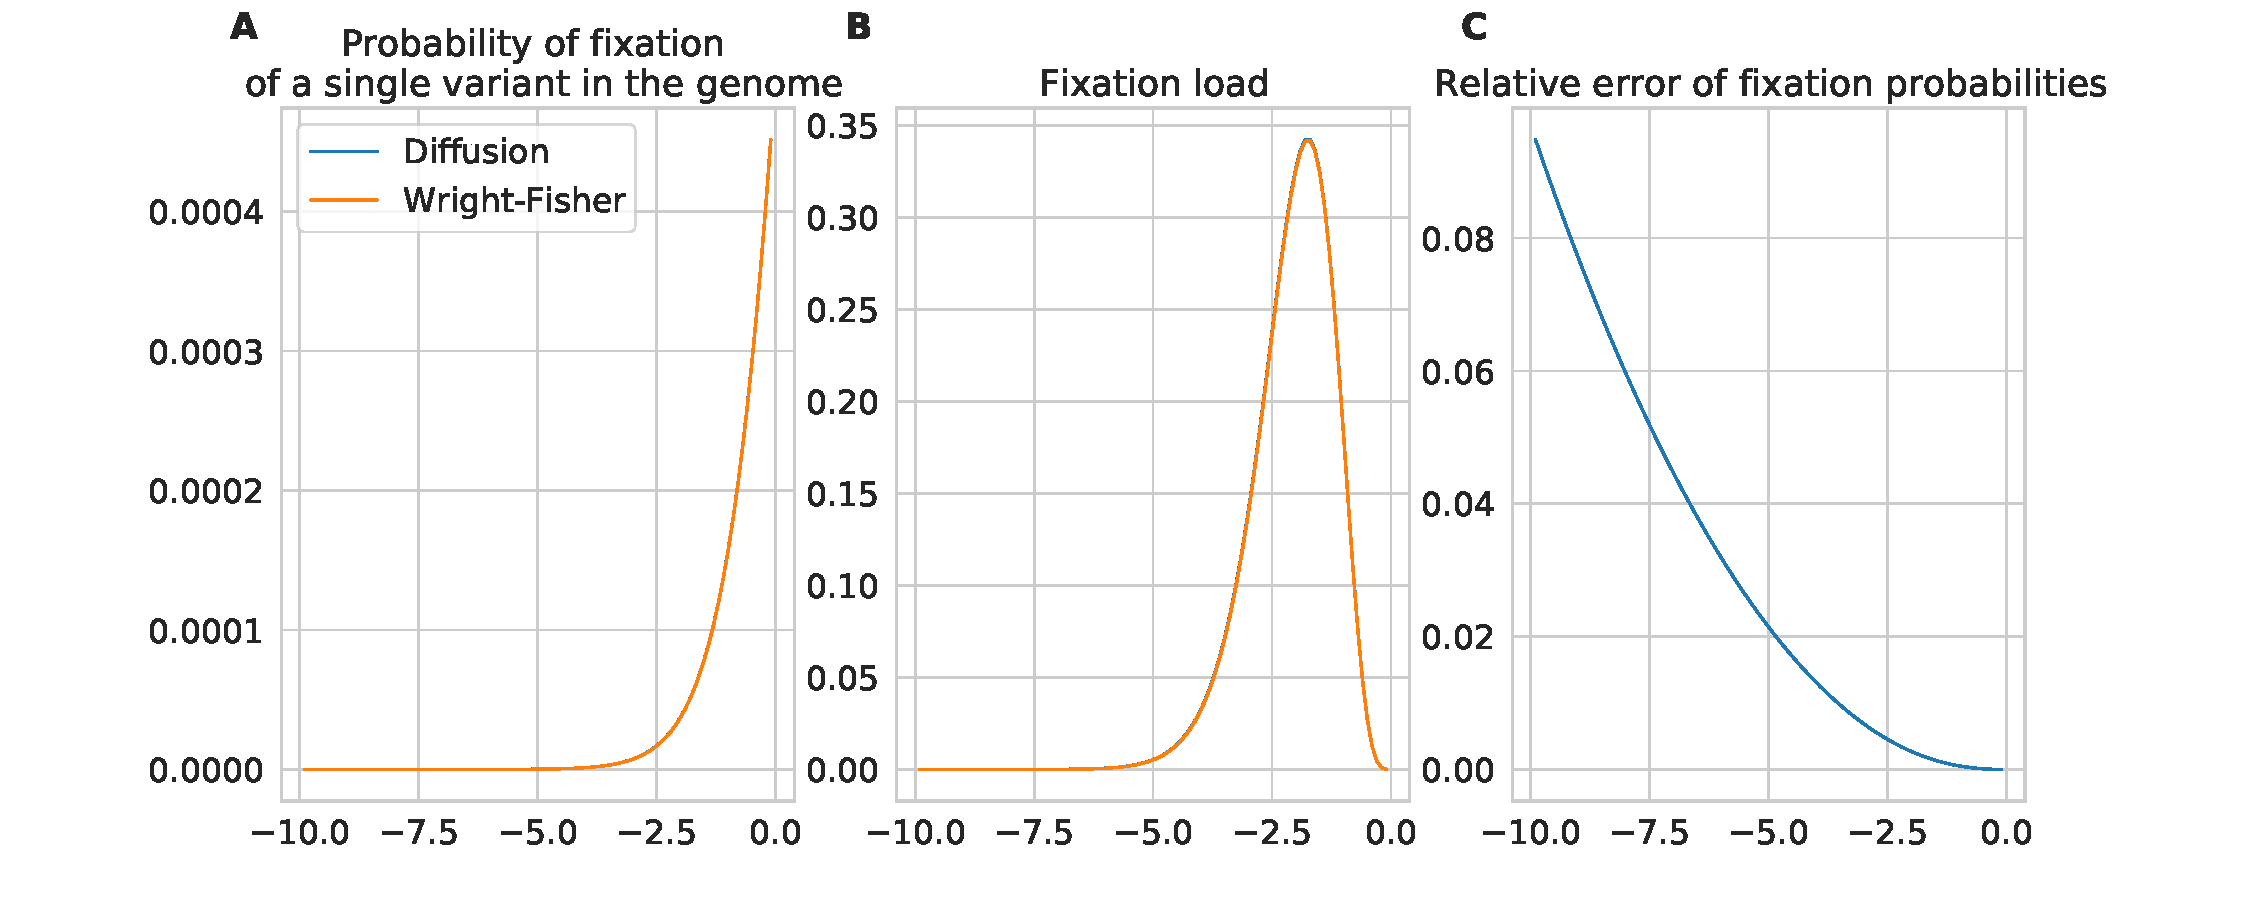
\includegraphics[width=\columnwidth]{fig/fixation_rate_N_1000.pdf}

    \caption{(A) Fixation probability, (B) fixation load, and (C) relative error between the
    diffusion and Wright-Fisher models for N=1000.}

  \label{fig_apx_fixation_1000}

\end{figure}
%\subsection{Missing lineages}

\begin{figure}
  \centering
  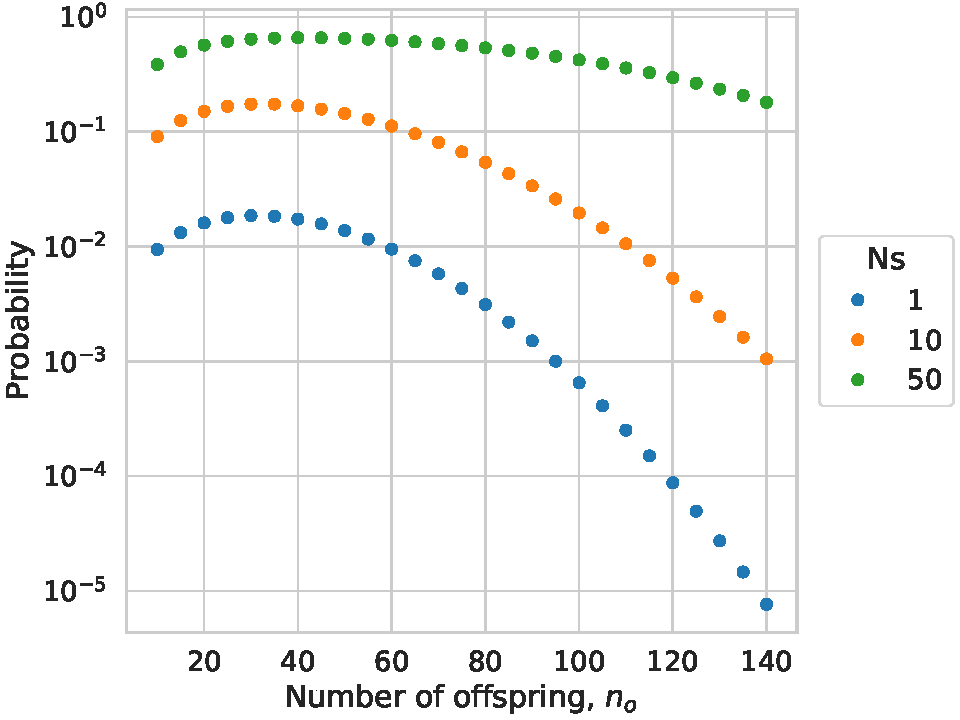
\includegraphics[width=\columnwidth]{fig/missing.pdf}

  \caption{Probability that there are more contributing parents than offspring: $n_p > n_o$ when
    every allele is derived (worst case). Calculated as $1-\sum_{i_o} \mathbf{Q}_{n_o}{(i_p,
    i_o)}$, with $Q$ defined in equation \ref{eq_truncated}, with $N=1000$. Each panel shows an
    increasing order of the jackknife approximation. Transparent points show sample sizes below the
    critical point, $2Ns$.}

  \label{fig_apx_missing}
\end{figure}

%\subsection{Quantiles of the Gaussian approximation}

%Figure \ref{fig_apx_critical_normal} shows the critical sample size for a given quantile of the normal
%approximation, as a function of the population-scaled selection coefficient. The $50^{\text{th}}$
%percentile corresponds to the mean calculated in equation \ref{eq_critical_sample} ($\approx 2Ns$).
%If we want to ascertain that the distribution is closed with increased confidence, we require a
%larger number of lineages. All curves assume $N=1000$.

\begin{figure}
  \centering
  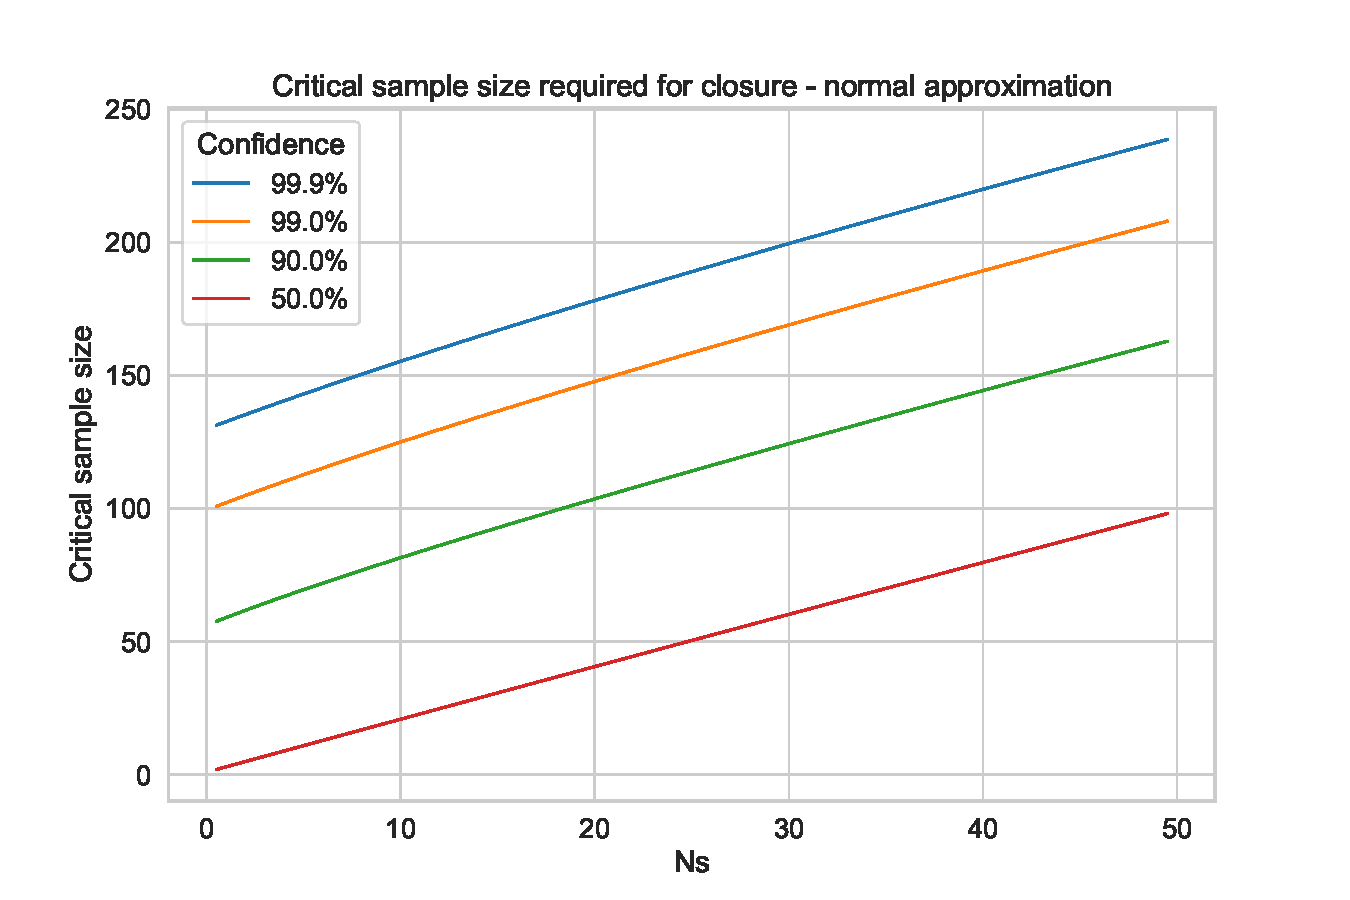
\includegraphics[width=\columnwidth]{fig/critical_normal.pdf}
  \caption{Critical sample size that is required to ensure that a given proportion of simulated
  draws are included, for a given closure confidence level. The
    $50^\text{th}$ percentile corresponds to the mean in the equation \eqref{eq_critical_sample}. Note that the
    normal approximation is invalid for $Ns=0$, where the occupancy distribution should be used. All
    lines are calculated with $N_e=1000$.}
  \label{fig_apx_critical_normal}
\end{figure}

\begin{figure}
  \centering
  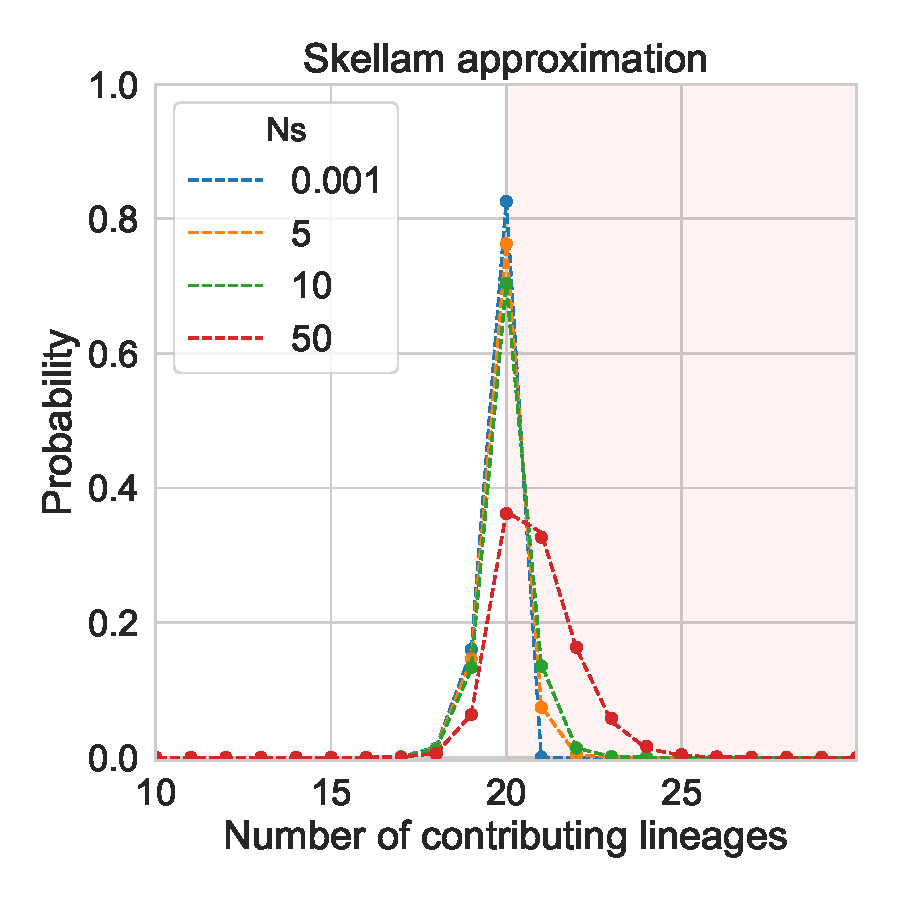
\includegraphics[width=\columnwidth]{fig/skellam.pdf}
  \caption{Skellam approximation to the number of required lineages where $n_o$ is small:
  $\frac{{n_o}^2}{2N} < 10$. The Skellam distribution describes the difference between the number
  of offspring lineages $n_o$, and parental lineages $n_p$. }
  \label{fig_apx_skellam}
\end{figure}

\begin{table}
    \centering
    \begin{tabular}{ c c r r r }
        N & Ns & $L$ & $L_{diffusion}$ & Relative error \\
        \hline
        $200$  & $0$  & $       0$ & $       0$ & $0\%$ \\
               & $1$  & $1.149e-8$ & $1.150e-8$ & $0.086\%$ \\
               & $5$  & $1.128e-8$ & $1.130e-8$ & $0.181\%$ \\
               & $10$ & $1.054e-8$ & $1.056e-8$ & $0.148\%$ \\
               & $20$ & $1.025e-8$ & $1.026e-8$ & $0.140\%$ \\
               & $50$ & $1.009e-8$ & $1.010e-8$ & $0.146\%$ \\
        \\
        $400$  & $0$  & $       0$ & $       0$ & $0\%$ \\
               & $1$  & $1.150e-8$ & $1.150e-8$ & $0.041\%$ \\
               & $5$  & $1.129e-8$ & $1.130e-8$ & $0.090\%$ \\
               & $10$ & $1.055e-8$ & $1.056e-8$ & $0.073\%$ \\
               & $20$ & $1.026e-8$ & $1.026e-8$ & $0.068\%$ \\
               & $50$ & $1.010e-8$ & $1.010e-8$ & $0.068\%$ \\
        \\
        $1000$ & $0$  & $       0$ & $       0$ & $0\%$ \\
               & $1$  & $1.150e-8$ & $1.150e-8$ & $0.016\%$ \\
               & $5$  & $1.130e-8$ & $1.130e-8$ & $0.036\%$ \\
               & $10$ & $1.056e-8$ & $1.056e-8$ & $0.028\%$ \\
               & $20$ & $1.026e-8$ & $1.026e-8$ & $0.027\%$ \\
               & $50$ & $1.010e-8$ & $1.010e-8$ & $0.026\%$ \\
        \\
        $2000$ & $0$  & $       0$ & $       0$ & $0\%$ \\
               & $1$  & $1.150e-8$ & $1.150e-8$ & $0.009\%$ \\
               & $5$  & $1.130e-8$ & $1.130e-8$ & $0.017\%$ \\
               & $10$ & $1.056e-8$ & $1.056e-8$ & $0.014\%$ \\
               & $20$ & $1.026e-8$ & $1.026e-8$ & $0.014\%$ \\
               & $50$ & $1.010e-8$ & $1.010e-8$ & $0.013\%$ \\
        \end{tabular}

    \caption{\label{tab_apx_load} Genetic load under the allele frequency
    spectra from present study ($L$), and the diffusion approximation
    ($L_{diffusion}$), with sample size $n=200$ individuals. Load calculated as
    $L=\sum_i s \frac{i}{n} \phi(i)$, relative error is
    $\frac{L-L_{diffusion}}{L}\times100\%$. }

\end{table}

\subsection{Deriving the recursion on the transition matrices}
\label{subsec_apx_tpm_deriv}

The transition matrices $\mathbf{T}_{r}\Coalc{i_p}{n_p}{i_o}{n_o}$ are equal to sampling
probabilities $P(\ms_{n_o}(i_o, n_p, r) | \CC{(i_p,n_p)} ),$ where $\ms_{n_o}(i_o,n_p, r)$ is the
event that $i_o$ of the first $n_o$ offspring carry the derived allele, that the $r$
draws following the $n_o$th drawn offspring are rejected, and that at the end of the $r$th
rejection we have drawn exactly $n_p$ parents . Our goal here is to derive a recursion
over the last event $\ell$. We characterize the last draw event in terms of whether it is
successful ($\sigma_\ell=1$) or not ($\sigma_\ell=0$); whether it draws a derived allele
($\gamma_\ell=1$) or not ($\gamma_\ell=0$), and whether it draws a previously undrawn parental
allele ($\delta_\ell=1$) or not ($\delta_\ell=0$).

With this notation in place, we can write our recursion as:
 \begin{equation}
  P( \ms_{n_o}(i_o, n_p, r) | \CC{(i_p,n_p)} ) = \sum_\ell P( \ms_{n_o}(i_o, n_p, r),\ell | \CC(i_p,n_p) ) .
 \end{equation}

Now that we have explicitly specified the last draw $\ell,$ we can remove the corresponding
information from event $\ms,$

\begin{equation}
  P(\ms_{n_o}(i_o, n_p, r) | \CC{(i_p,n_p)} ) = \sum_\ell \sum_{r' \in R_\ell} P(\ms_{n'_o}(i_o',
  n'_p, r'),\ell | \CC{(i_p,n_p)} ) .
\end{equation}
where $i_o' = i_o-\gamma_\ell$,  $n_o' = n_o-\sigma_\ell,$ $i'_p= i_p - \delta_\ell \gamma_\ell,$  and $n'_p  = n_p - \delta_\ell$ represent the
counts of derived and total alleles among the offspring and parents prior to the last draw.
 The number of failures $r'$ can take more than one value if the last draw was a success,
so that

\begin{equation}
  R_\ell = \begin{cases}
    \{r-1\}    & \text{for } \sigma_\ell = 0, \\
    \mathbb{N} & \text{for } \sigma_\ell = 1.
  \end{cases}
\end{equation}

We can further simplify the notation by defining shorthand for events prior to the last draw,
 $\ms' = \ms_{n'_o}(i_o', n'_p, r)$, and $\CC' = \CC{(i'_p,n'_p)}$, and after the
last draw $\ms = \ms_{n_o}(i_o, n_p, r)$, and $\CC = \CC{(i_p,n_p)}$

The event  $\CC'$ is fully determined by  $\CC$ and $\ell$, so that we can write

\begin{equation}
  \begin{split}
    \mathbf{T}_{r}\Coalc{i_p}{n_p}{i_o}{n_o} = P(\ms| \CC) &= \sum_\ell \sum_{r' \in R_\ell}
    P(\ms',\ell | \CC) \\
    &=\sum_\ell \sum_{r' \in R_\ell}P( \ms',\ell, \CC' |\CC) \\
    &=\sum_\ell \sum_{r' \in R_\ell}P(\ell | \ms', \CC', \CC ) P( \ms'| \CC', \CC)  P(\CC' |\CC) \\
    &=\sum_\ell \sum_{r' \in R_\ell}P(\ell | \ms', \CC', \CC ) P( \ms'| \CC')       P(\CC' |\CC) \\
    &=\sum_\ell \sum_{r' \in R_\ell}P(\ell | \ms', \CC', \CC ) P(\CC' |\CC)  \mathbf{T}_{r'}\Coalc{i'_p}{n'_p}{i'_o}{n'_o}
  \end{split}
\end{equation}
where the third line is an application of the chain rule and the fourth line uses the independence
of primed events on the last draw.  We now simply need to enumerate all the distinct types of
events for the last draw and compute the corresponding probabilities, which we do on Figure
\ref{fig_rec_selection_dynamic_fail}.

\subsection{Distribution on the number of parental lineages}

%With sufficiently large sample sizes, the missing probability can be made
%very small. In addition, we can use the jackknife approximation \citep{JouganousEtAl2017} to improve
%model performance.

%The transition probability matrices can be useful in numerical approaches, but they provide little
%intuition about the general behaviour of the model. In the following sections, we derive
%approximations to the process to gain more insight.

\subsection{Distribution of number of sampled lineages}
\label{parent_distribution}

To disentangle the effects of drift and selection, in addition to tracking the parental and
offspring lineages, we also define $n_g$ as the number of gametes sampled in the process (Fig.
\ref{fig_schematic_gametes}). The difference $n_g-n_o \ge 0$ depends on the number of selective
deaths, whereas the difference $n_p-n_g \le 0$ depends on the number of coalescent events.

\begin{figure}
  \centering
  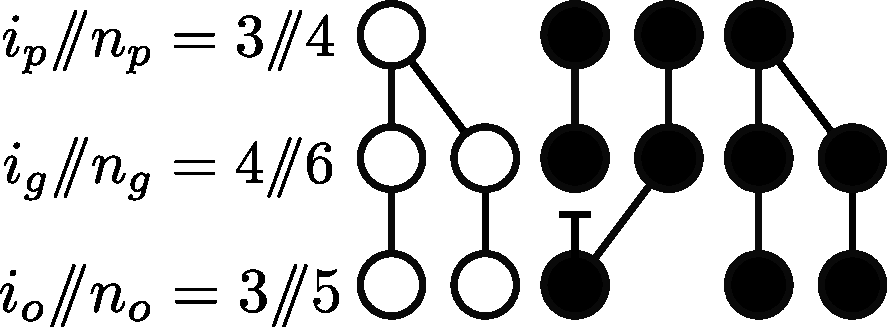
\includegraphics[width=\columnwidth]{fig/schematic-gametes.pdf}

  \caption{\label{fig_schematic_gametes}
    An extension of figure \ref{fig_schematic}, with the addition of the gamete
    "generation", with $n_g$ gametes, of which $i_g$ are derived.  }
\end{figure}

To get an analytical expression for the probability of missing lineages, in the worst-case scenario
where all the parental alleles are derived, we consider the probability that $n_p$ parents have been
sampled,

\begin{equation}
  \begin{aligned}
    \label{eq_conditional}
    P_{n_o}(n_p) = \sum_{n_g} P_{n_o}(n_p | n_g)P_{n_o}(n_g)
  \end{aligned}
\end{equation}
where $n_p$ and $n_g$ is the number of sampled parents and gametes, respectively (Fig.
\ref{fig_schematic}C).

The distribution over the number of gametes, $n_g$, is given by the negative binomial,
parameterized by the number of successes $n_o$, and the probability of a successful draw is $1-s$.

\begin{equation}
  \begin{aligned}
    \label{eq_neg_binomial_trials}
    P_{n_o}(n_g) = \binom{n_g-1}{n_o-1}(1-s)^{n_o}(s)^{n_g-n_o}.
  \end{aligned}
\end{equation}
Given $n_g$, the number of parental lineages $n_p$ follows the modified occupancy distribution
(also known as the Arfwedson distribution) \citep{Wakeley2009,ONeill2019,JohnsonEtAl2005}:

\begin{equation}
  \begin{aligned}
    \label{eq_occupancy}
    P(n_p|n_g) = \frac{S_2(n_g,n_p) N!}{(N-n_p)! N^{n_g}}
  \end{aligned}
\end{equation}
where $S_2(n_g,n_p)$ is a Stirling number of the second kind, which is the number of ways to
partition $n_g$ gametes into $n_p$ parents (see \cite{JohnsonEtAl2005} section 10.4 for a thorough
treatment).
The occupancy distribution requires exchangeability of the alleles, which is satisfied by the
condition that all parental alleles are derived.

Combining the two distributions together through equation \ref{eq_conditional}, we get:
\begin{equation}
  \begin{aligned}
    \label{eq_lineages_in_past}
    P(n_p|n_o) = \sum_{n_g=1}^{\infty} \frac{S_2(n_g,n_p) N!}{(N-n_p)! N^{n_g}} \binom{n_g-1}{n_o-1}(1-s)^{n_o}(s)^{n_g-n_o}
  \end{aligned}
\end{equation}

We did not find an analytical expression for this sum, but it can be computed
efficiently using methods presented in \citep{ONeill2019}. Figure \ref{fig_combined}A (dotted line) shows
the distribution of the number of contributing parental lineages for several selection coefficients
with $n_o=200$.
As the strength of selection
is increased, we begin requiring larger numbers of lineages, while with increasing sample size,
there is a decrease in required lineages due to coalescent events.

\begin{figure}
  \centering
  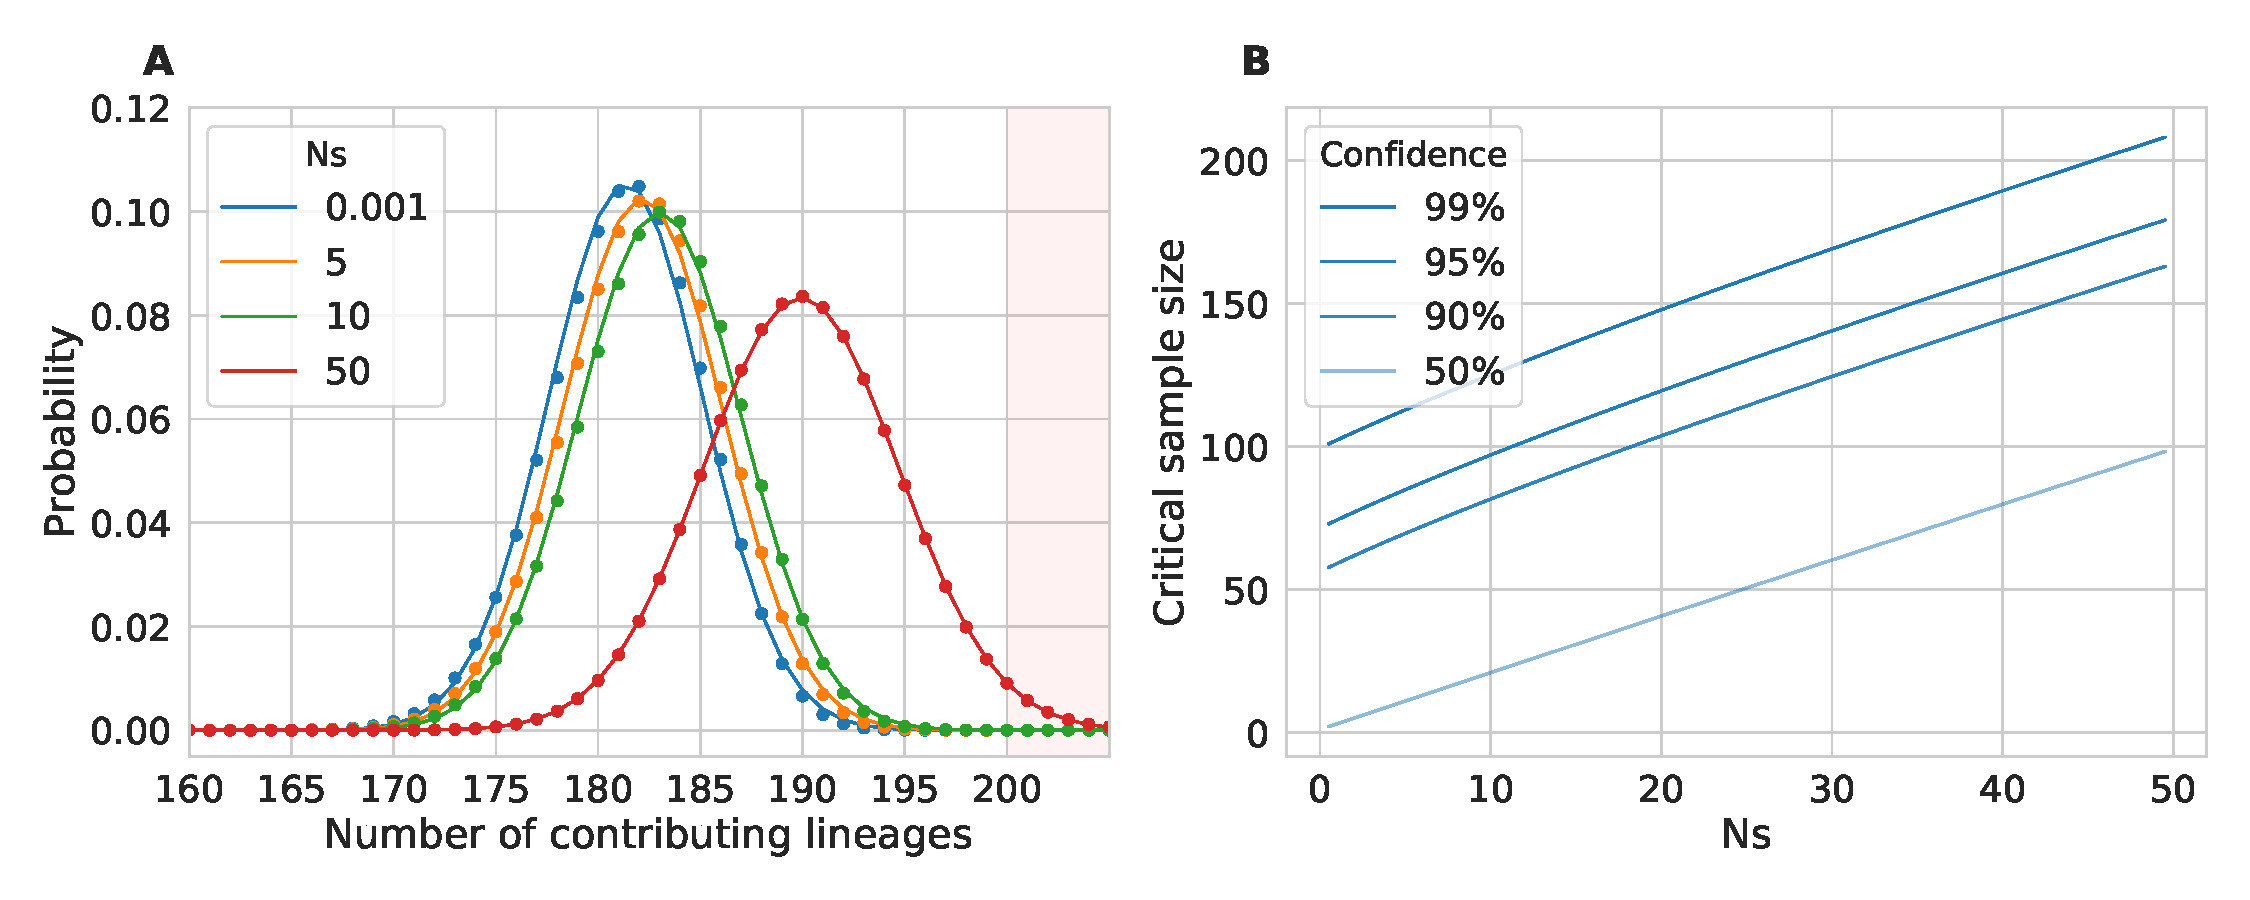
\includegraphics[width=\columnwidth]{fig/combined.pdf}
  \caption{\textbf{A} The distribution of number of required lineages with $n_0=200$. Shaded
    red area shows missing probability, where $n_p > n_o$. Points represent the exact probability one
    generation into the past (Eq. \ref{eq_lineages_in_past}), solid lines - Gaussian approximation.
     \textbf{B} Sample size ($n_o$) as a fraction of population size ($N$)
    such that we have $99\%$ confidence that no lineages are missing, derived from the Gaussian
    approximation. The dotted line indicates regimes where the Gaussian approximation is likely inaccurate.
     In both panels, $N=1000$.}
  \label{fig_combined}
\end{figure}

\subsection{Gaussian approximation}
\label{subsec_gaussian}

The distribution in equation \ref{eq_lineages_in_past} can quickly be calculated numerically, but
provides little intuition. We therefore compute the
expectation and variance of this distribution, and show that it can be accurately approximated by
Skellam and Gaussian distributions in useful parameter regimes.

Using the law of total expectation, we can write the expectation $E[n_p-n_o | n_o]$ as
\begin{equation*}
  \begin{aligned}
    E[n_p-n_o | n_o] &=        E[n_p | n_o]       - n_o \\
                     &=E_{n_g} E_{n_p}[n_p | n_g] - n_o.
  \end{aligned}
\end{equation*}

The expectation over $n_p$ is simply that of the occupancy distribution \cite{Wakeley2009}.

\begin{equation*}
  \begin{aligned}
    \label{eq_lineages_derive}
    \hat{E}[n_p -n_o | n_o]
    & =   E_{n_g}\left[N\left[1-\left(1 - \frac{1}{N} \right)^{n_g} \right]\right]- n_o\\
    & =   N-N  E_{n_g}\left[\left(1 - \frac{1}{N} \right)^{n_g} \right] -n_o.
  \end{aligned}
\end{equation*}

As mentioned above, the number of selective deaths, $n_g-n_o$ follows a negative binomial
distribution with success probability $1-s$. We can use the moment generating function of the
negative binomial to compute the expectation of $k^{n_g}$ for any constant $k$:

%\begin{equation}
%E_{n_g}[k^{n_g}] = k^{n_o}  \left(\frac{1-s}{1-sk}\right)^{n_o}.
%\label{eq_identity}
%\end{equation}
%\sgcomment{I believe that the general case is:}
\begin{equation}
  E_{n_g}[k^{n_g}] = k^{n_o}  \left(\frac{1-s}{1-sk}\right)^{n_o}.
  \label{eq_identity}
\end{equation}

Thus we can write:

% \begin{equation}
%\begin{aligned}
% \label{eq_gauss_mean}
% \hat{E}[n_p -n_o | n_o] &= N-N\left( 1 - \frac{1}{N} \right)^{n_o}\left( \frac{1-s}{1-s \left( 1 - \frac{1}{N} \right)}\right)^{n_o}-n_o.
%\end{aligned}
% \end{equation}

%\sgcomment{General case}

\begin{equation}
  \begin{aligned}
    \label{eq_gauss_mean}
    \hat{E}[n_p -n_o | n_o] &= N-N\left( 1 - \frac{1}{N} \right)^{n_o}\left( \frac{1-s}{1-s \left( 1 - \frac{1}{N} \right)}\right)^{n_o}-n_o.
  \end{aligned}
\end{equation}

Taking the terms of order up to $\frac{1}{N}$ gives

\begin{equation}
    \hat{E}[n_p-n_o | n_o] \approx n_o  s - \frac{n_o (n_o-1) }{2N}.
\end{equation}

We thus have the usual interplay of selection and drift. Solving for $ \hat{E}[n_p -n_o | n_o]\leq0$
yields, to leading order,

\begin{equation}
  n_o^* \ge 2N s.
\end{equation}

This represents a critical sample size (Fig.
\ref{fig_apx_critical_normal}) where there is more drift than selection events, on average.
The next section outlines a similar approach to compute the variance of this distribution, $\operatorname{Var}[n_p-n_o | n_o].$

\subsubsection{Variance of number of contributing lineages}
\label{subsec_apx_variance}

We can obtain the variance of the distribution of the number of parental lineages $P(n_p | n_o)$ by using the law of total variance:

\begin{equation}
  \label{eq_apx_var}
\Var\left[n_p-n_o \right] = \Var_{n_g}\left[E\left[n_p-n_o | n_g \right]\right]+  E_{n_g}\left[Var\left[n_p-n_o | n_g \right]\right]
\end{equation}
As previously, we are assuming that all the parental alleles are derived.
The expectation in the first term can be derived from the occupancy distribution and the identity
\ref{eq_identity}:
\begin{equation}
\begin{split}
\Var_{n_g}\left[E\left[n_p-n_o | n_g \right]\right] &= \Var_{n_g}\left[E\left[n_p| n_g \right]\right] \\
&= \Var_{n_g}\left[N\left(1-(1-\frac{1}{N})^{n_g} \right) \right] \\
&= N^2 \Var_{n_g}\left[(1-\frac{1}{N})^{n_g} \right] \\
&= N^2 \left( E_{n_g}\left[(1-\frac{1}{N})^{2n_g} \right] - E_{n_g}\left[(1-\frac{1}{N})^{n_g} \right]^2\right) \\
&= N^2 \Bigg[ \left(1-\frac{1}{N}\right)^{2n_o} \left(\frac{1-s}{1-s \left(1-\frac{1}{N}\right)^2}\right)^{n_o} \\
&- \left(1-\frac{1}{N}\right)^{2n_o} \left(\frac{1-s}{1-s \left(1-\frac{1}{N}\right)}\right)^{2n_o}\Bigg] \\
\end{split}
\end{equation}
The variance of the second term of Equation \eqref{eq_apx_var} is the variance of the modified occupancy
distribution \cite{JohnsonEtAl2005}:

\begin{equation}
\begin{split}
	E_{n_g}\left[Var\left[n_p-n_o | n_g \right]\right] 
	&= E_{n_g}\Big[N ((N - 1) (1 - 2/N)^{n_g} + (1 - 1/N)^{n_g} \\
	&- N (1 - 1/N)^{2 n_g}) \Big] \\
	&= N (N-1) \left( \frac{ (1-s)\left( 1-\frac{2}{N} \right) }{ 1-s\left( 1-\frac{2}{N} \right) } \right)^{n_o} + \\
	&+ N \left( \frac{(1-s)\left( 1-\frac{1}{N} \right)}{1-s\left( 1-\frac{1}{N} \right)}\right)^{n_o} - \\
	&- N^2 \left( \frac{(1-s)\left( 1-\frac{1}{N} \right)^2}{1-s\left( 1-\frac{1}{N} \right)^2}\right)^{n_o} \\
\end{split}
\end{equation}

Combining the two terms in Equation \eqref{eq_apx_var}, we get

\newcommand{\vara}[1]{\left(1-\frac{#1}{N}\right)}
\newcommand{\varb}[1]{\left(\frac{1-s}{1-s #1}\right)}

\begin{equation}
  \begin{aligned}
	  \Var[n_p-n_o | n_o] &= N^2\Bigg( \vara{1}^{2n_o}\varb{\vara{1}^2}^{n_o} \\ 
	  &-\vara{1}^{2n_o}\varb{\vara{1}}^{2n_o} \Bigg) + \\
	  &+ N (N-1) \Bigg( \frac{ (1-s)\left( 1-\frac{2}{N} \right) }{ 1-s\left( 1-\frac{2}{N}
	  \right) } \Bigg)^{n_o} \\
	  &+ N \left( \frac{(1-s)\left( 1-\frac{1}{N} \right)}{1-s\left( 1-\frac{1}{N} \right)}\right)^{n_o} \\ 
	  &- N^2 \left( \frac{(1-s)\left( 1-\frac{1}{N} \right)^2}{1-s\left( 1-\frac{1}{N} \right)^2}\right)^{n_o}.
  \label{eq_exact_var}
  \end{aligned}
\end{equation}

Taking series expansion in Mathematica \citep{Mathematica}, we can show that

\begin{equation}
  \begin{aligned}
    \operatorname{Var}[n_p-n_o | n_o] &= n s + \frac{n (n-1)}{2 N_e}  + \cdots
  \end{aligned}
\end{equation}
where missing terms are of at least second order in products of  $s$, $\frac{n}{N}$,  and
$\frac{1}{N}.$ The code is available in the github repository.

\subsection{Simplifying Gaussian approximation}
\label{subsec_apx_gauss}
Given a $z$ for the change in the number of lineages of $ z = \frac{-\mu}{\sqrt{\sigma^2}},$
we use $\mu=\left(  n_zs - \frac{n_z(n_z-1)}{2N} \right)$ and $\sigma = \sqrt{n_zs +
\frac{n_z(n_z-1)}{2N}}$ from Equations \ref{eq_lineages_approx} and \ref{eq_gauss_var} to obtain a bound for $n_z$:


\begin{equation}
\begin{aligned}
  z &= \frac{-\left(  n_zs - \frac{n_z(n_z-1)}{2N} \right)}	{\sqrt{n_zs + \frac{n_z(n_z-1)}{2N}}} \\
  z &\approx \frac{\frac{n_z^2}{2N} - n_z s}	{\sqrt{n_zs + \frac{n_z^2}{2N}}} \geq \frac{\frac{n_z^2}{2N} - n_z s}{n_z / \sqrt{N}} \\
 \end{aligned}
\end{equation}
 The latter inequality uses the fact that we are in the regime where the expected number of drift events is larger than the number of
 selection events. Thus $\left(n_zs +
\frac{n_z^2}{2N} \right) \leq \left(\frac{n_z^2}{2N} + \frac{n_z^2}{2N} \right)$.

 This can now be trivially solved for $n_z$ to yield
 \begin{equation}
  n_z \leq 2\sqrt{N}z + 2Ns
\end{equation}

\subsection{Construction of transition probability matrices with multiple generations}
\label{subsec_apx_multi}

Multi-generation transition matrices can simply be computed by iterating equation \eqref{eq_recur}.
Assuming, for simplicity, that the population sizes and selection coefficients are constant over the
last two generations, and using matrix products to account for sums over the number $i_p$ of
parental derived alleles, we find
\begin{equation}
\begin{split}
\afs{n_o}{t} &=  \sum_{n_p=1}^{n_{p,max}}  \mathbf{T}_{n_o,n_p}     \afs{n_p}{t-1}\\
&=  \sum_{n_p=1}^{n_{p,max}} \mathbf{T}_{n_o,n_p}     \sum_{n'_p=1}^{n'_{p,max}}  \mathbf{T}_{n_p,n'_p}\afs{n'_p}{t-2}\\
&=  \sum_{n'_p=1}^{n'_{p,max}}  \left(\sum_{n_p=1}^{n_{p,max}} \mathbf{T}_{n_o,n_p}
    \mathbf{T}_{n_p,n'_p} \right)\afs{n'_p}{t-2}\\
&\equiv  \sum_{n'_p=1}^{n'_{p,max}}  T^{(2)}_{n_p',n_o} \afs{n'_p}{t-2}.
\end{split}
\end{equation}
where $n'_{p'}$ is the number of sampled lineages in the grandparental generation, and $n_{p,max}$
and $n'_{p,max}$ are the maximum number of sampled parental alleles considered in the parental and
grandparental generations, respectively.  We can choose $n_{p,max}>n_o$ and $n_{p,max} = n_o$  to
preserve closure of the moment equation while allowing for drift to cancel out selection events over
the course of two generations.

Since each matrix product takes $O(n_o n_p n_{p'})$, and there are at most $O(n_{p,max})$ such
products, the computation of this matrix product takes at most $O(n_o n_{p,max}^2 n_{p'}).$ This
scaling can be improved upon in numerical implementations by summing only over values of $n_p$ that
contribute appreciably.  In addition, we need to build the matrices $T_{n_p', n_p}$ themselves.  In
the recursive approach, the computation of the matrix for the largest sample includes the
computation of matrices for smaller sample sizes, so the computation time is at most that of the
largest possible matrix, $O(r_{max} n_{p,max}^2, n_{p',max}^2).$ In the exact formulation of our
model, $n_p$ can be as large as $ r_{max} n_o,$ however this would require every draw to be rejected
by selection and only contribute terms of order $s^{n_o r_{max}}.$ A numerically appropriate cutoff
for a given $n_o$ and $s$ can be computed dynamically by keeping track of the proportion of
unaccounted-for lineages. In most practical applications with $s<0.1$ we expect that choosing, e.g.,
$n_{p,max}=  2 n_o$ would provide excellent convergence, hence an overall scaling of   $O(r_{max}
n_{o}^4)$ for the construction of the matrices and $O(n_o^4)$ for the matrix product.  Thus a naive
construction of a transition matrix over $g$ generations would require  $O( (g + r_{max} ) n_o^4).$



\end{document}
